\documentclass[11pt,a4paper]{article}

\usepackage[utf8]{inputenc}
\usepackage[T1]{fontenc}
\usepackage[margin=2.3cm]{geometry}
\usepackage{graphicx}
\usepackage{float}
\usepackage{subcaption}
\usepackage{enumitem}
\usepackage{xcolor}
\usepackage{booktabs}
\usepackage[hidelinks]{hyperref}

\graphicspath{{./fotos/}}
\setlist{itemsep=2pt, topsep=4pt}

\newcommand{\key}[1]{\texttt{\textbf{#1}}}
\newcommand{\menu}[1]{\textsf{#1}}
\newcommand{\fig}[3]{%
  \begin{figure}[H]
    \centering
    \includegraphics[width=#2\linewidth]{#1}
    \caption{#3}
  \end{figure}}

\title{\textbf{3D Model}\\[4pt]
\large Step-by-step documentation of the modeling process}
\author{Jonathan Felipe L\'opez Nu\~nez\\
\small \href{mailto:jolopezn@unal.edu.co}{\texttt{jolopezn@unal.edu.co}}\\[6pt]
\small Professor: Andres Ricardo Arevalo Murillo}
\date{November 6, 2026}

\begin{document}
\maketitle

\tableofcontents
\newpage

%=====================================================================
\section{Introduction}
%=====================================================================
This document presents the step-by-step 3D modeling workflow of Snorlax in Blender, developed for the creation of the final \texttt{.obj} model and its multi-material setup.

The visual concept and modeling were inspired by the character design featured in the video \href{https://youtu.be/6IQGmw8v8Gc?si=VUwGOW6OvqKOC7GY}{\emph{``[Blender Character Modeling] Snorlax Joined the Akatsuki''}} by Poly Crafted (Figure~\ref{fig:inspiration}). The original project scope intended to include both the Akatsuki cloak and the Magikarp sword. However, because a significant amount of time was invested in learning Blender fundamentals, tools, modifiers, and modeling techniques, the work was concentrated on achieving a clean, detailed model of Snorlax complete with the rogue ninja headband, metal plate, and engraved symbol.

\begin{figure}[H]
  \centering
  
\includegraphics[width=0.85\linewidth]{01_inspiration_video.png}
  \caption{Inspiration model from the YouTube video \href{https://youtu.be/6IQGmw8v8Gc?si=VUwGOW6OvqKOC7GY}{\emph{``[Blender Character Modeling] Snorlax Joined the Akatsuki''}} by Poly Crafted.}
  \label{fig:inspiration}
\end{figure}

%=====================================================================
\section{Reference setup}
%=====================================================================
Before modeling, reference drawings of the character were loaded into the
scene so that every part could be traced with the correct proportions.

\begin{enumerate}
  \item \menu{Add $\rightarrow$ Image $\rightarrow$ Reference} was used to
        import a front view and a side view of the character.
  \item The front image was aligned with the \emph{front orthographic} view
        (\key{Numpad 1}) and the side image with the \emph{right
        orthographic} view (\key{Numpad 3}), both centered on the world
        origin.
  \item The references were grouped in a collection called
        \emph{Referencia} so they could be hidden or locked easily, and their
        opacity was lowered so the model is visible through them.
\end{enumerate}

\fig{08_reference_images.png}{0.85}{Reference images imported into the scene.}
\fig{09_reference_front_side.png}{0.85}{Front and side references aligned at the origin.}

%=====================================================================
\section{Body}
%=====================================================================
\subsection{Base shape}
\begin{enumerate}
  \item A cube was added (\menu{Add $\rightarrow$ Mesh $\rightarrow$ Cube})
        and scaled to fit the outline of the body in the front view.
  \item A \textbf{Subdivision Surface} modifier was added so the cube
        becomes a smooth, rounded volume while keeping a low number of
        editable vertices.
  \item In \textbf{Sculpt Mode}, the \emph{Grab} brush was used with
        symmetry on the X axis to push and pull the surface until the
        silhouette matched the reference: a wide, pear-shaped body that is
        heavier at the bottom.
\end{enumerate}

\fig{10_base_cube_over_reference.png}{0.7}{Initial cube placed over the front reference.}
\fig{12_body_sculpt_grab.png}{0.85}{Shaping the body with the Grab brush in Sculpt Mode (X symmetry enabled).}

\subsection{Head}
A second rounded object was added above the body and adjusted in the same way
(scaling in Object Mode and editing vertices in Edit Mode) until it matched the
head outline in both views.

\begin{figure}[H]
  \centering
  \begin{subfigure}{0.48\linewidth}
    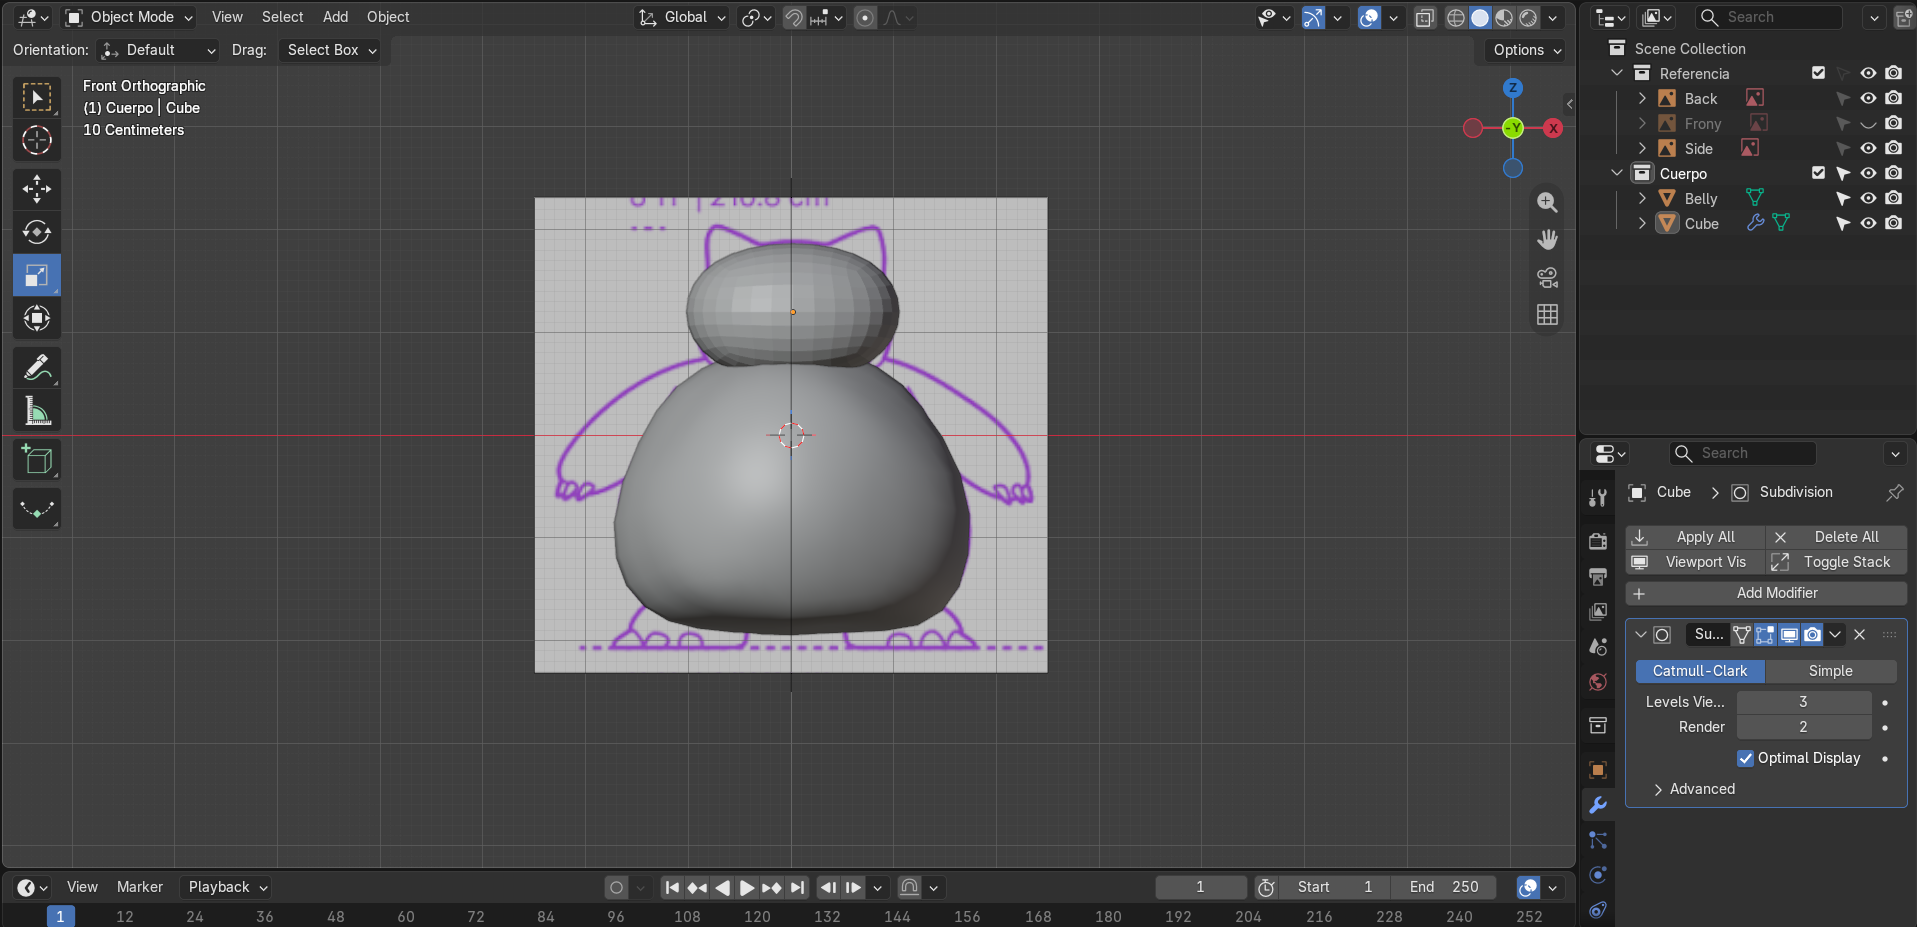
\includegraphics[width=\linewidth]{14_head_sphere_added.png}
    \caption{Head volume added.}
  \end{subfigure}\hfill
  \begin{subfigure}{0.48\linewidth}
    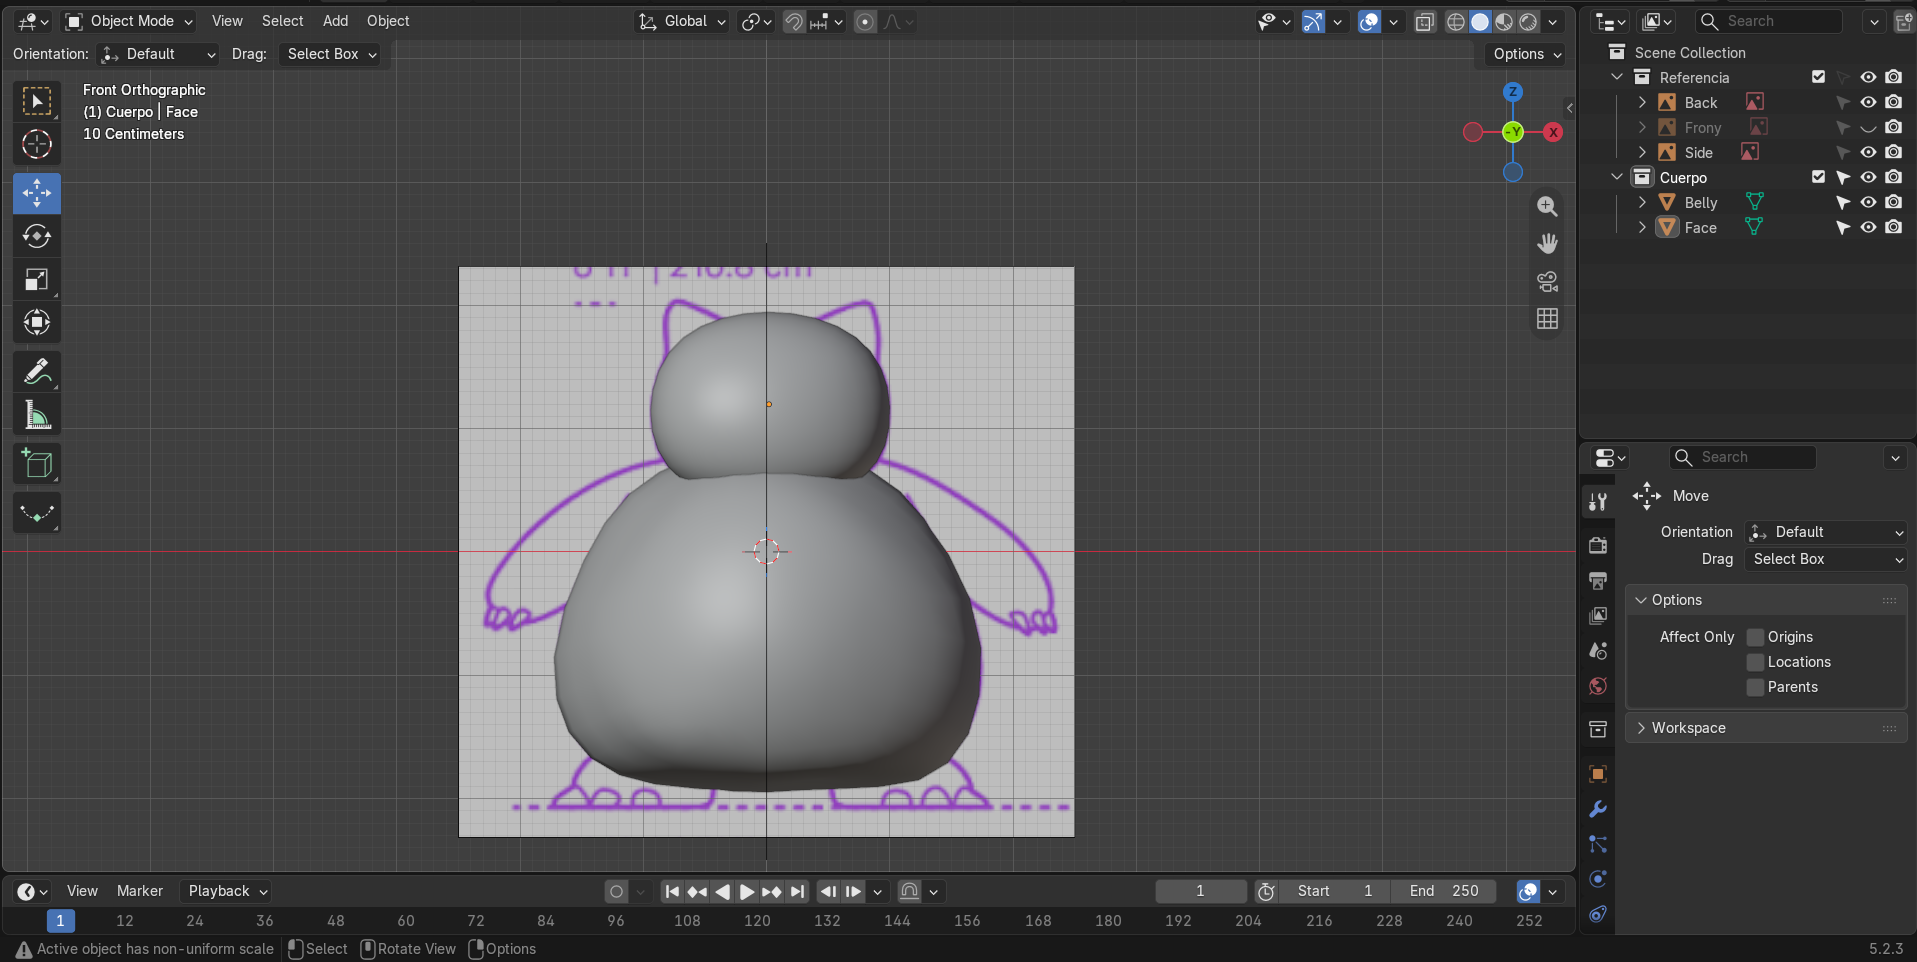
\includegraphics[width=\linewidth]{15_body_head_blocked.png}
    \caption{Body and head blocked out.}
  \end{subfigure}
  \caption{Blocking out the main volumes.}
\end{figure}

%=====================================================================
\section{Ears}
%=====================================================================
\begin{enumerate}
  \item A UV sphere was added near the top of the head.
  \item In Edit Mode, half of the sphere was selected and removed so that
        only a shell remained; this shell is the base of the ear. (An
        attempt to use \emph{Rip} (\key{V}) failed with the error
        \emph{``Cannot rip non-manifold vertices or edges''}, so the faces
        were deleted instead.)
  \item The shell was scaled and rotated to form the pointed ear shape and
        placed on the head.
  \item A \textbf{Mirror} modifier on the X axis created the second ear
        automatically.
\end{enumerate}

\begin{figure}[H]
  \centering
  \begin{subfigure}{0.48\linewidth}
    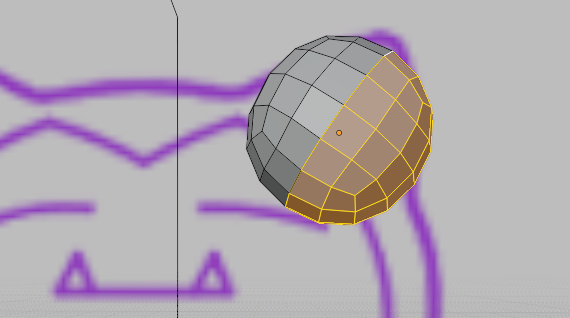
\includegraphics[width=\linewidth]{17_ear_half_sphere.png}
    \caption{Half of the sphere selected.}
  \end{subfigure}\hfill
  \begin{subfigure}{0.48\linewidth}
    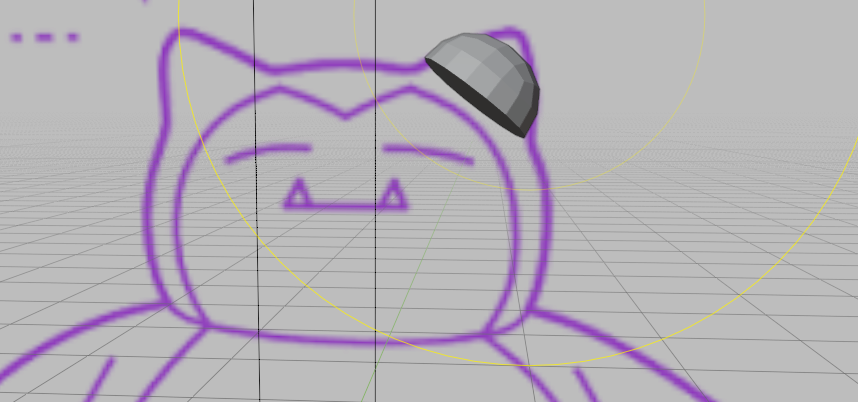
\includegraphics[width=\linewidth]{19_ear_placed.png}
    \caption{Ear placed on the head.}
  \end{subfigure}
  \caption{Modeling the ears.}
\end{figure}

%=====================================================================
\section{Feet and claws}
%=====================================================================
\begin{enumerate}
  \item Each foot was made from a flattened sphere placed at the bottom of
        the body, following the side reference.
  \item A \textbf{Mirror} modifier (X axis) duplicated the foot on the other
        side so both feet always stay symmetric.
  \item The toes were modeled with small cubes. In Edit Mode, the tip faces
        were selected and extruded with \key{E}
        (\emph{Extrude Region and Move}) to create pointed claws.
\end{enumerate}

\begin{figure}[H]
  \centering
  \begin{subfigure}{0.48\linewidth}
    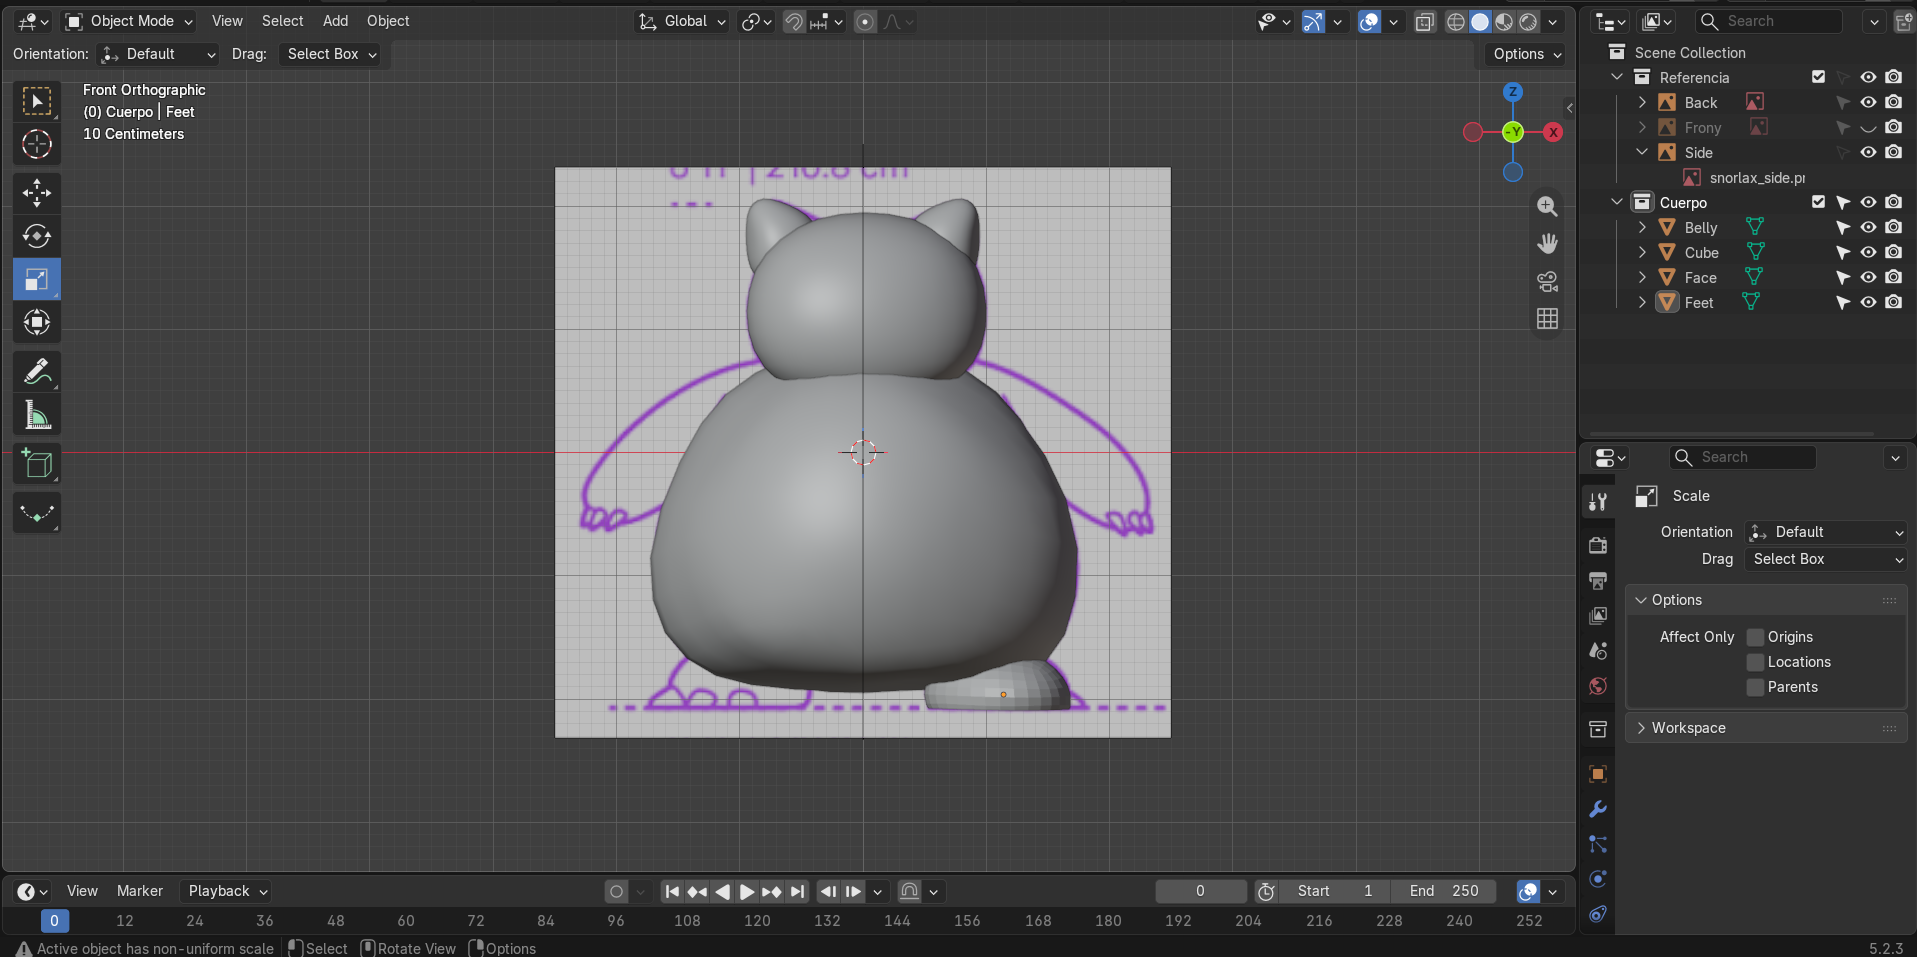
\includegraphics[width=\linewidth]{21_feet_added.png}
    \caption{Feet added.}
  \end{subfigure}\hfill
  \begin{subfigure}{0.48\linewidth}
    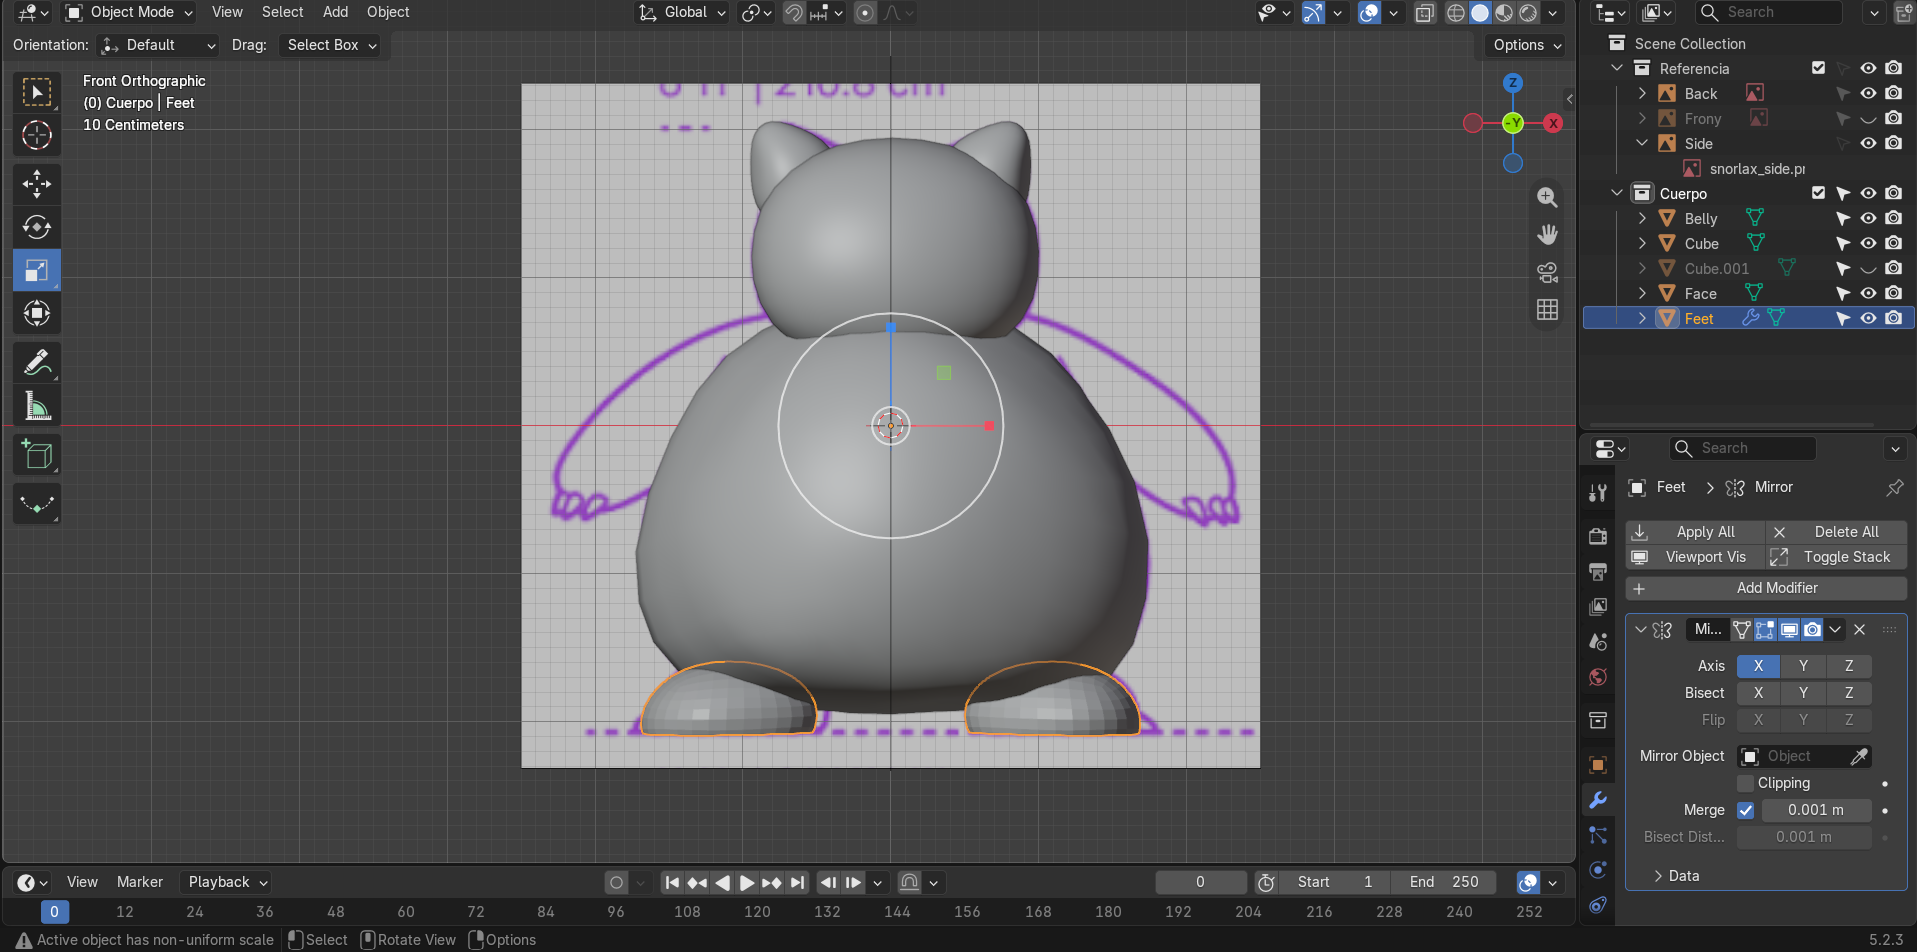
\includegraphics[width=\linewidth]{22_feet_mirror.png}
    \caption{Mirror modifier for symmetry.}
  \end{subfigure}
  \caption{Feet.}
\end{figure}

\begin{figure}[H]
  \centering
  \begin{subfigure}{0.48\linewidth}
    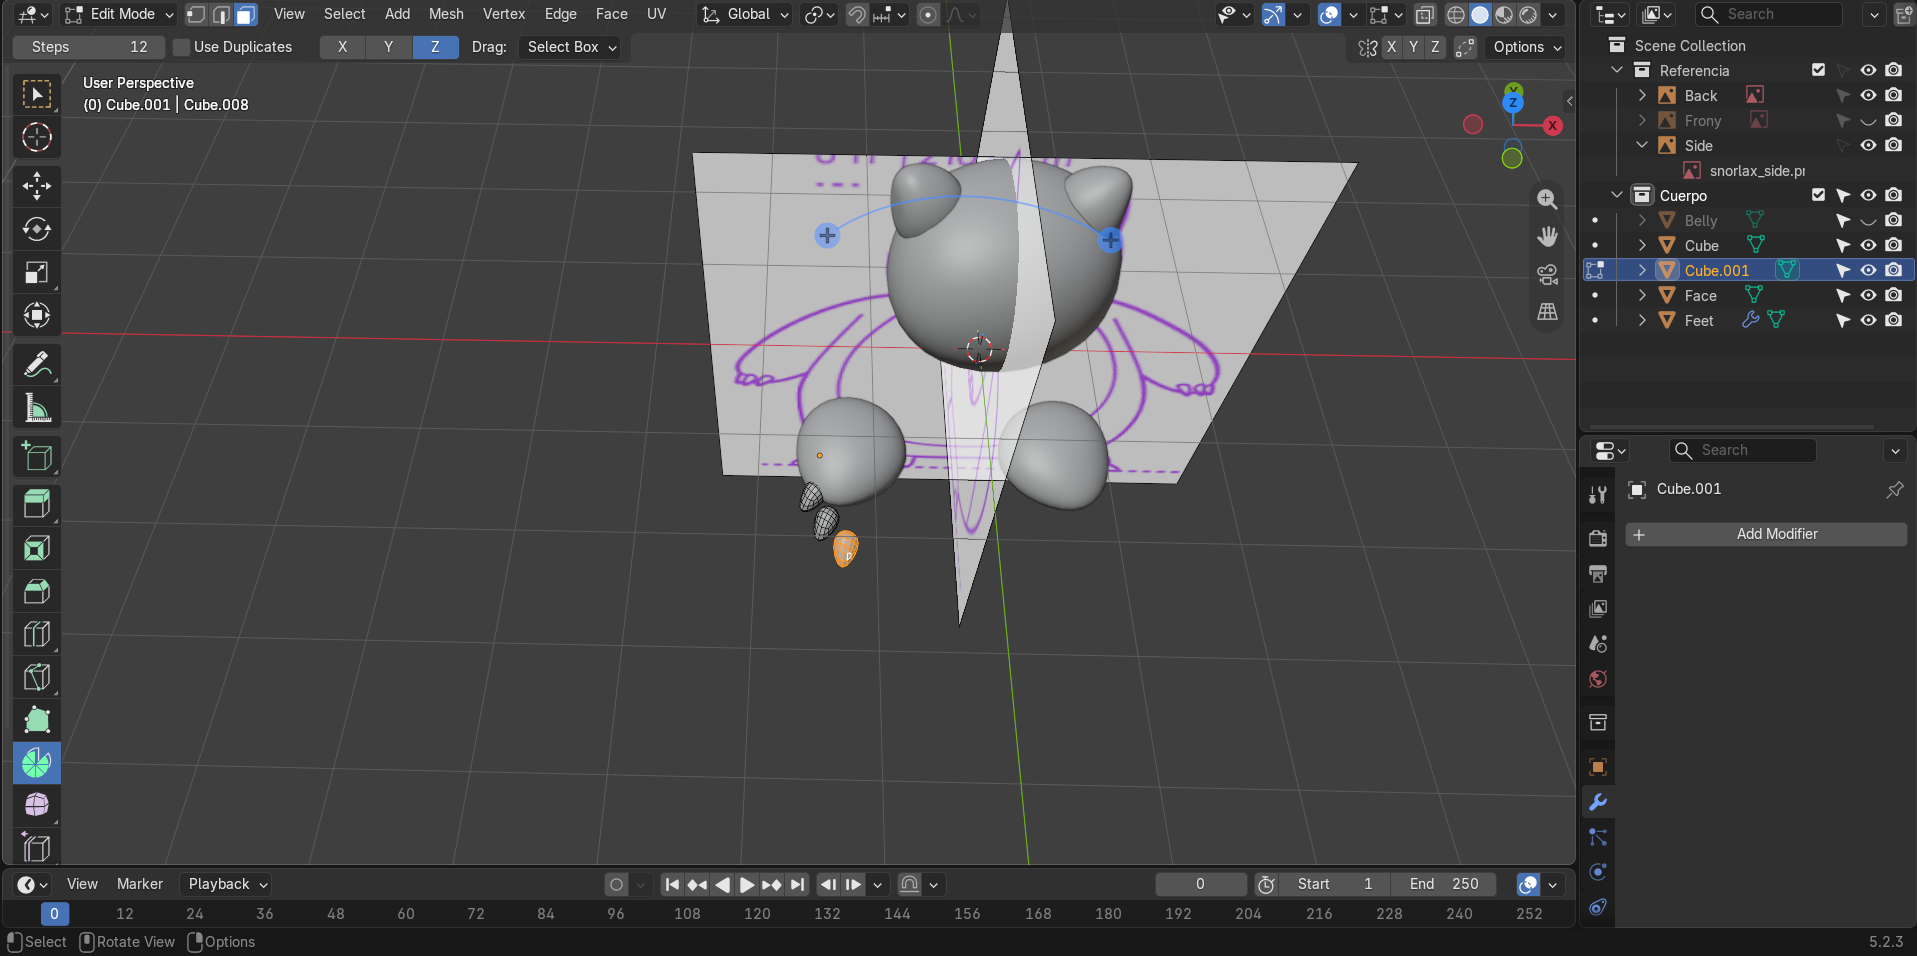
\includegraphics[width=\linewidth]{24_toes_symmetry.png}
    \caption{Toes positioned with symmetry.}
  \end{subfigure}\hfill
  \begin{subfigure}{0.48\linewidth}
    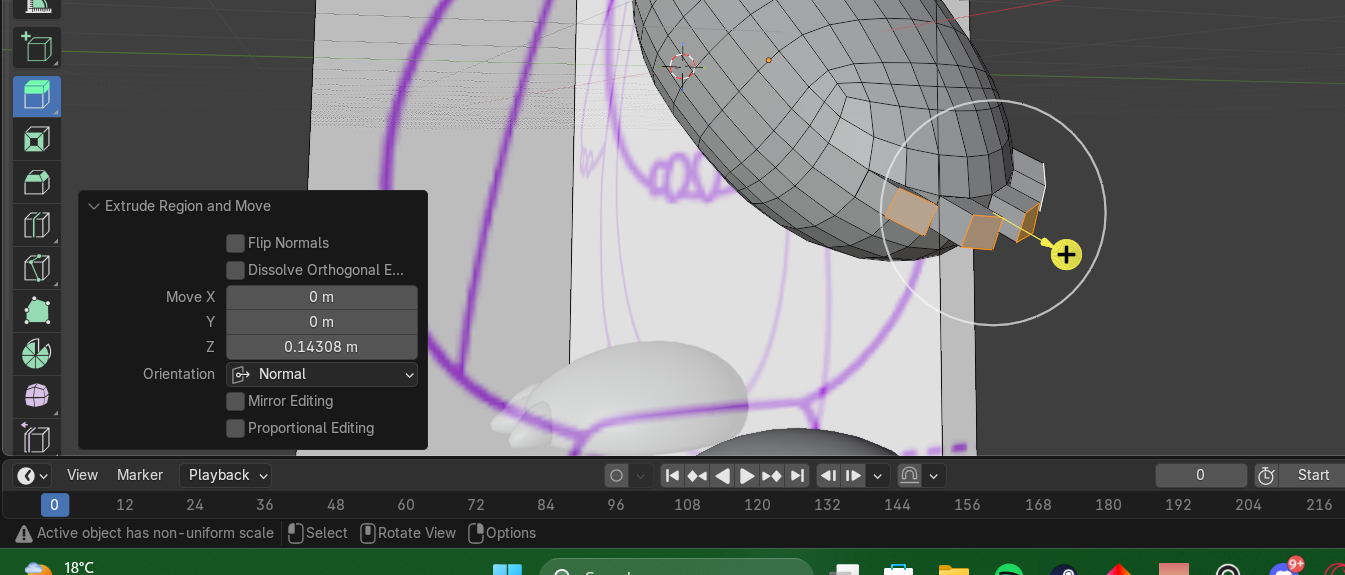
\includegraphics[width=\linewidth]{29_claw_extrude.png}
    \caption{Extruding the claw tips (\key{E}).}
  \end{subfigure}
  \caption{Toes and claws.}
\end{figure}

%=====================================================================
\section{Arms and hands}
%=====================================================================
\begin{enumerate}
  \item Each arm started as an elongated sphere rotated to follow the
        reference.
  \item In Sculpt Mode the arm was shaped with the Grab brush to make it
        thicker at the shoulder and thinner at the wrist.
  \item Small claws were added at the end of each hand using the same
        extrusion technique as the feet.
  \item The arm was mirrored to the other side.
\end{enumerate}

\begin{figure}[H]
  \centering
  \begin{subfigure}{0.48\linewidth}
    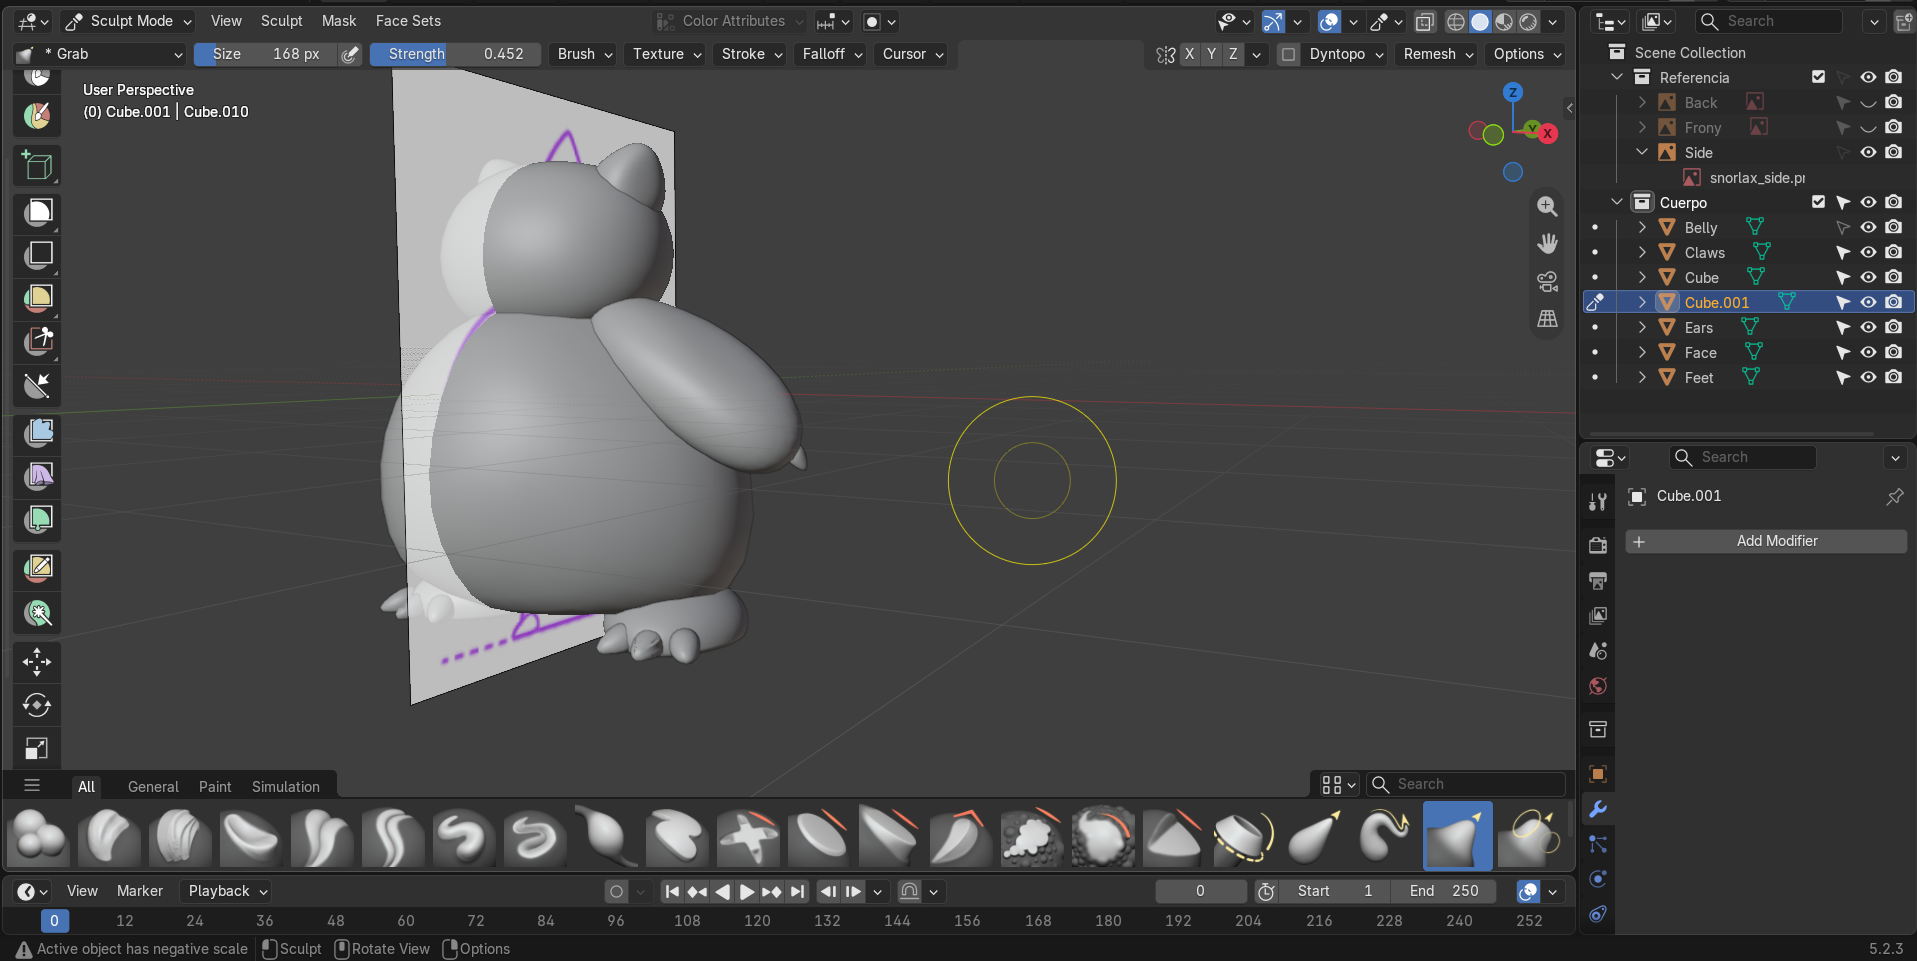
\includegraphics[width=\linewidth]{33_arm_sculpt.png}
    \caption{Sculpting the arm.}
  \end{subfigure}\hfill
  \begin{subfigure}{0.48\linewidth}
    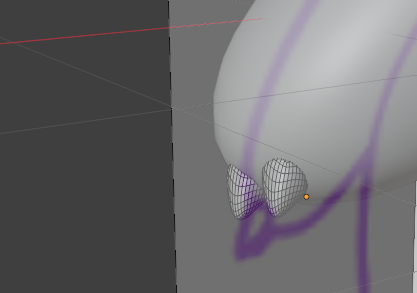
\includegraphics[width=\linewidth]{34_hand_claws.png}
    \caption{Hand claws.}
  \end{subfigure}
  \caption{Arms.}
\end{figure}

\fig{39_body_arms_complete.png}{0.6}{Complete body with arms, feet and ears.}

%=====================================================================
\section{Belly}
%=====================================================================
The belly needs a different color from the rest of the body.
\begin{enumerate}
  \item In Edit Mode with face selection (\key{3}), the front faces of the
        body that form the belly were selected.
  \item They were duplicated and separated into their own object
        (\key{Shift+D}, then \key{P} $\rightarrow$ \menu{Selection}), so the
        belly can receive its own material and be adjusted independently.
\end{enumerate}

\begin{figure}[H]
  \centering
  \begin{subfigure}{0.48\linewidth}
    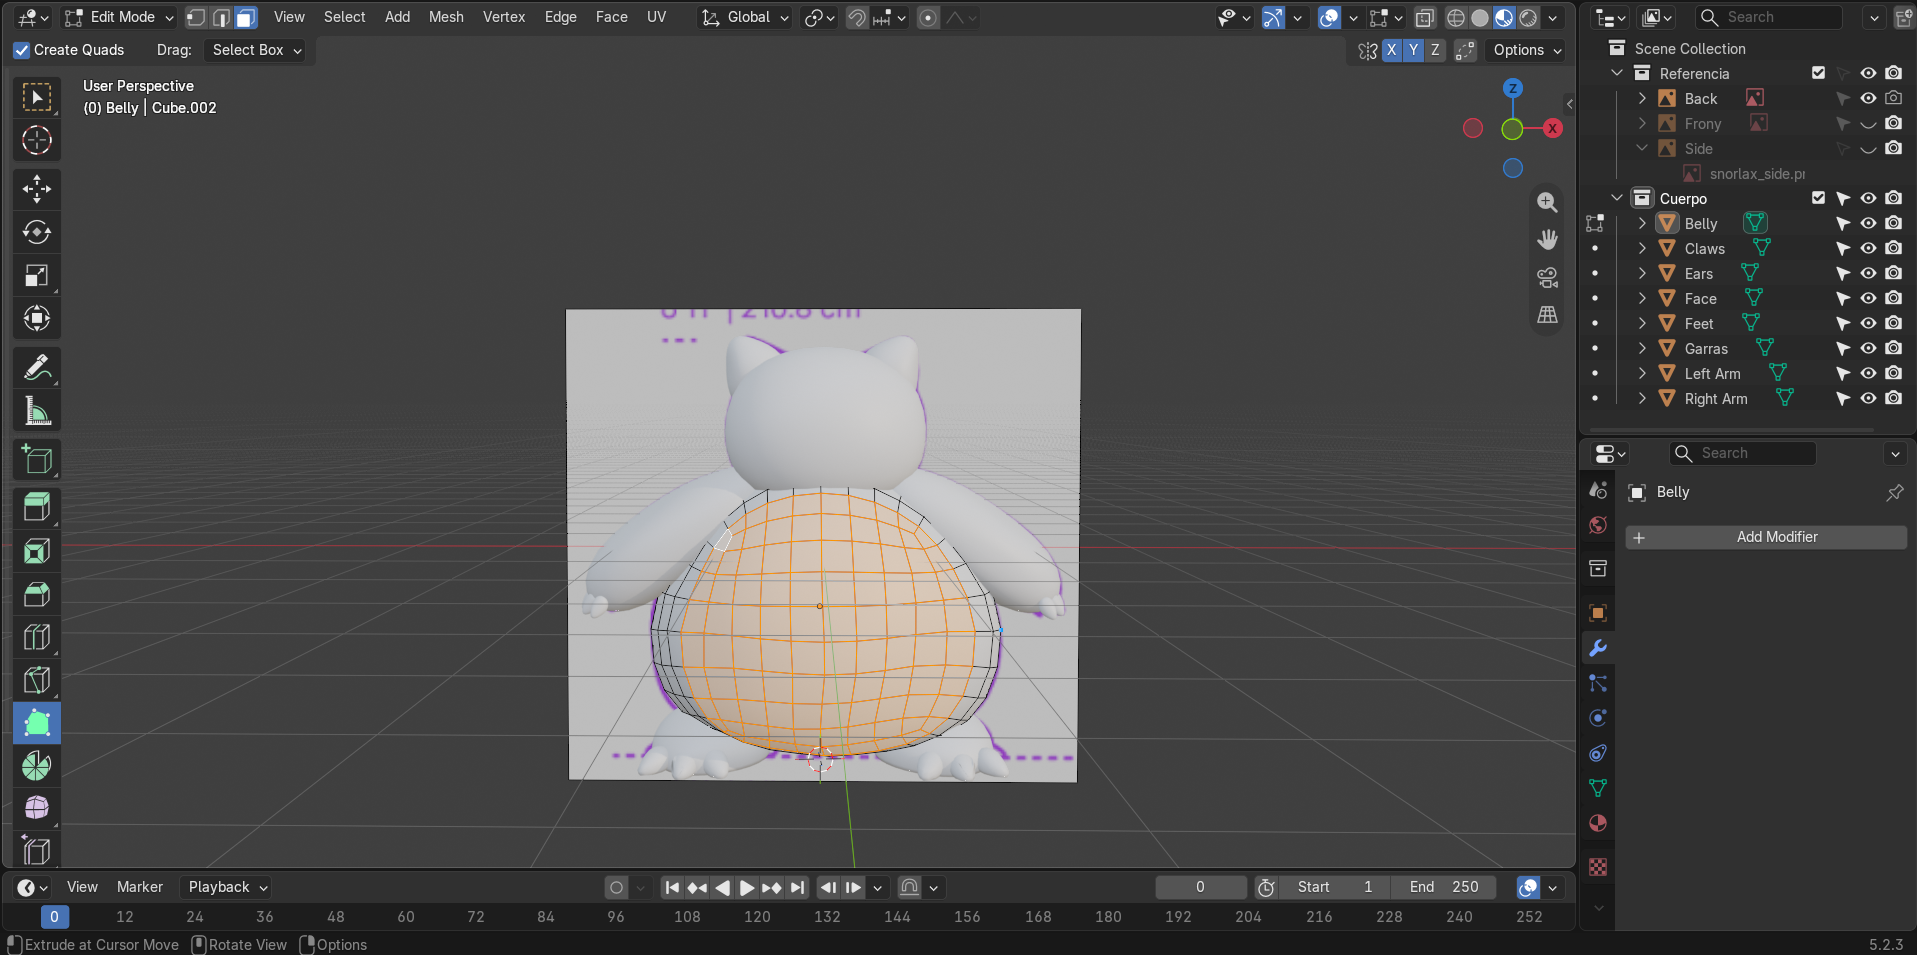
\includegraphics[width=\linewidth]{40_belly_faces_selected.png}
    \caption{Belly faces selected.}
  \end{subfigure}\hfill
  \begin{subfigure}{0.48\linewidth}
    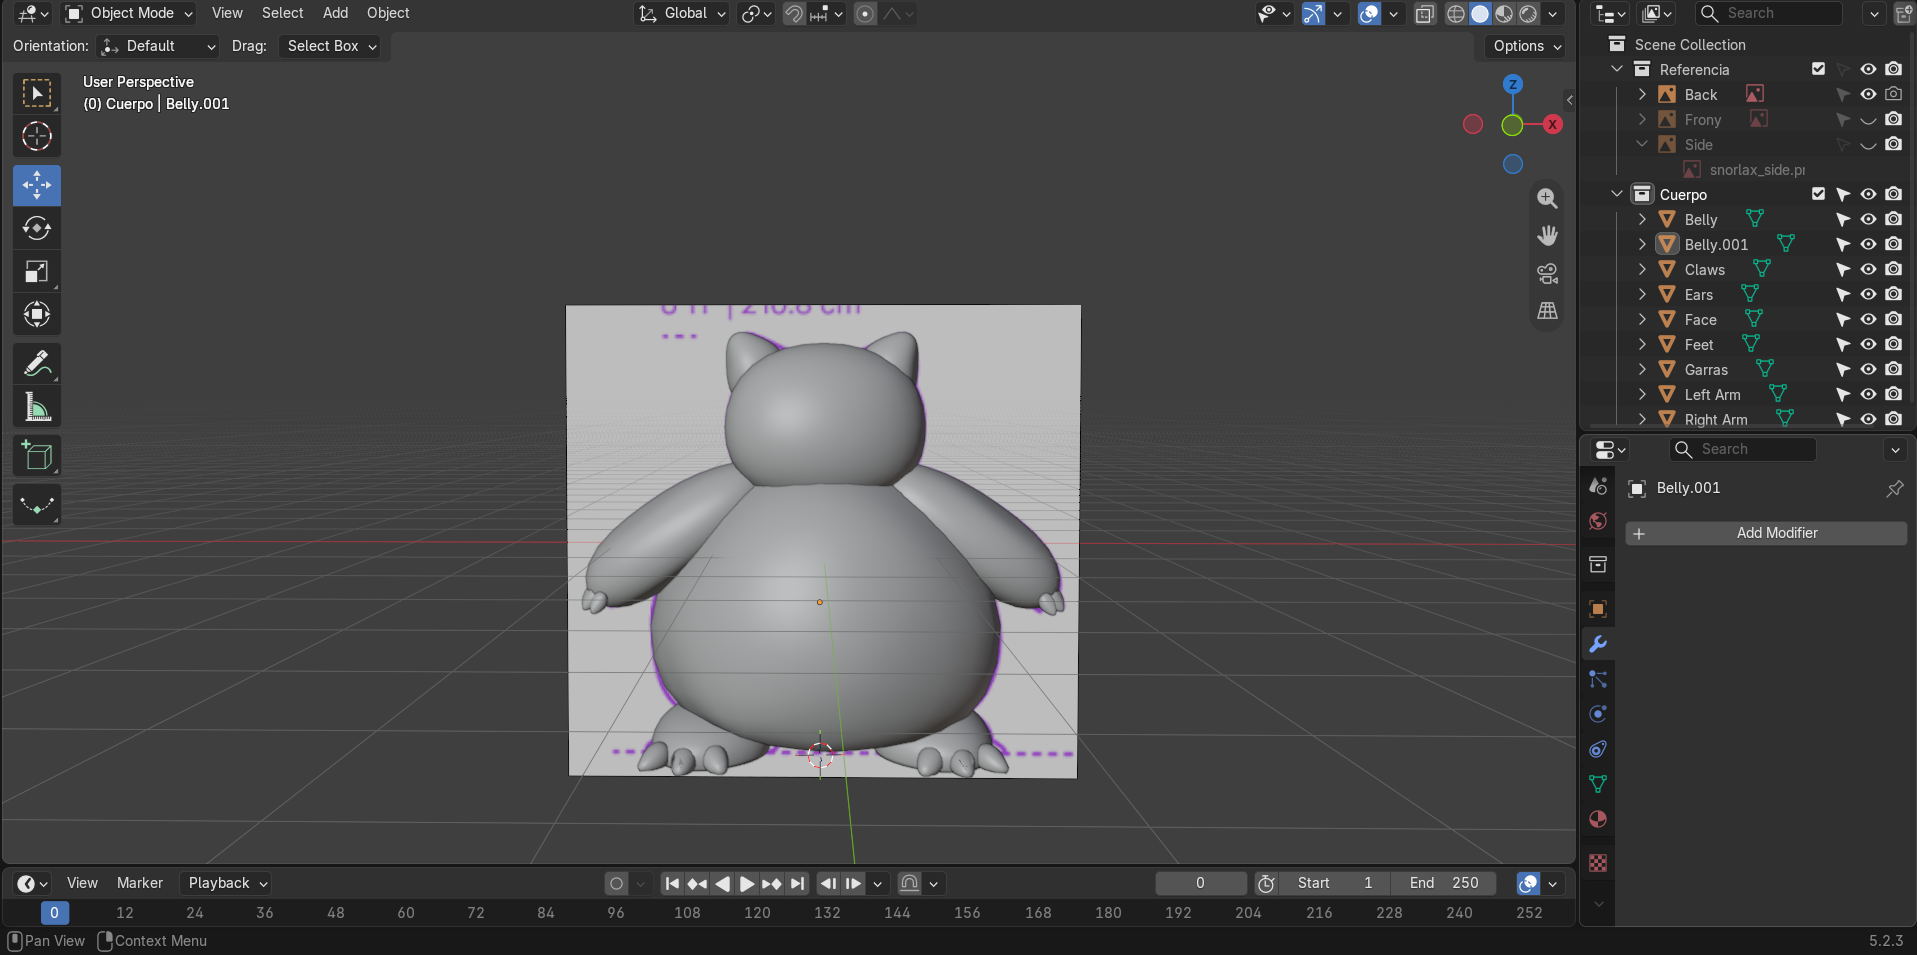
\includegraphics[width=\linewidth]{42_belly_separated.png}
    \caption{Belly as a separate object.}
  \end{subfigure}
  \caption{Belly.}
\end{figure}

%=====================================================================
\section{Materials}
%=====================================================================
Materials were created in the \menu{Material Properties} tab using the
\emph{Principled BSDF} shader:
\begin{itemize}
  \item \textbf{Body} -- blue, used for head, body, arms and ears.
  \item \textbf{Belly / face} -- off-white, used for the belly, face, feet
        and claws.
  \item \textbf{Metal} -- grey with high \emph{Metallic} and medium
        \emph{Roughness}, used for the headband plate and rivets.
  \item \textbf{Black} -- used for the eyes, mouth and plate symbol.
\end{itemize}

\fig{43_head_topology_color.png}{0.55}{Head with its material and visible topology.}

\begin{figure}[H]
  \centering
  \begin{subfigure}{0.32\linewidth}
    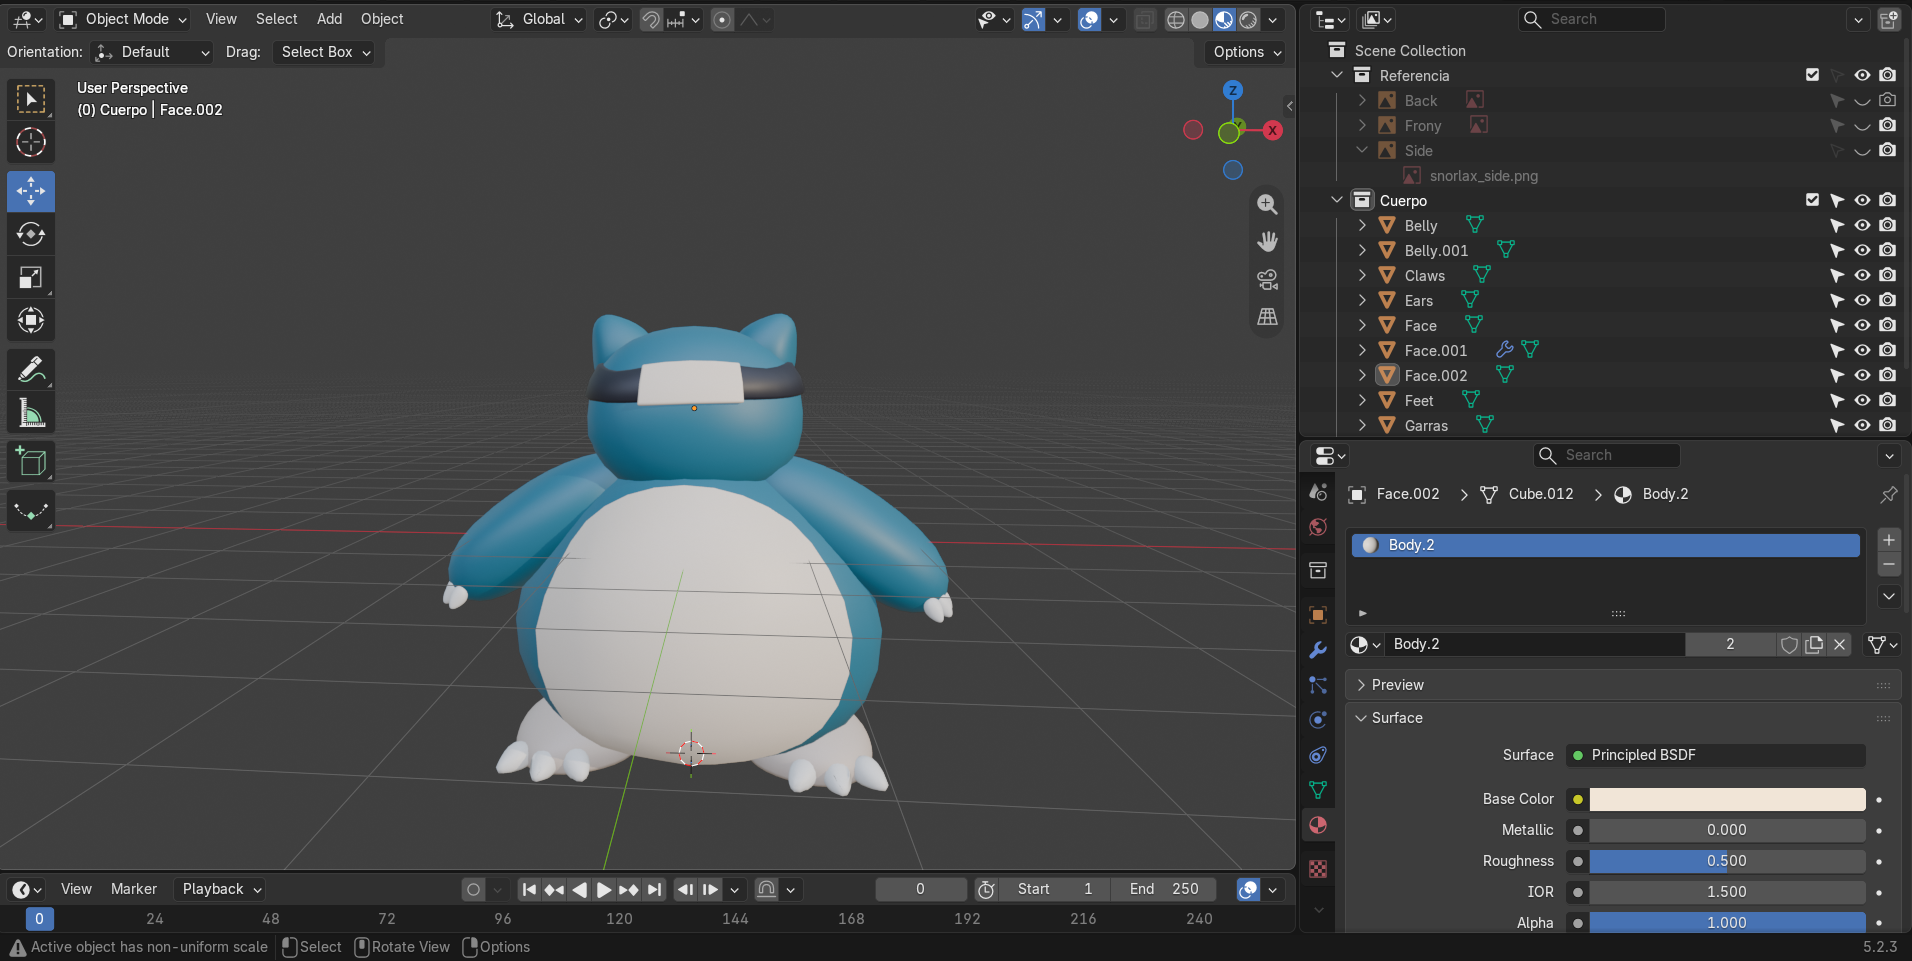
\includegraphics[width=\linewidth]{45_material_body_white.png}
    \caption{Off-white material.}
  \end{subfigure}\hfill
  \begin{subfigure}{0.32\linewidth}
    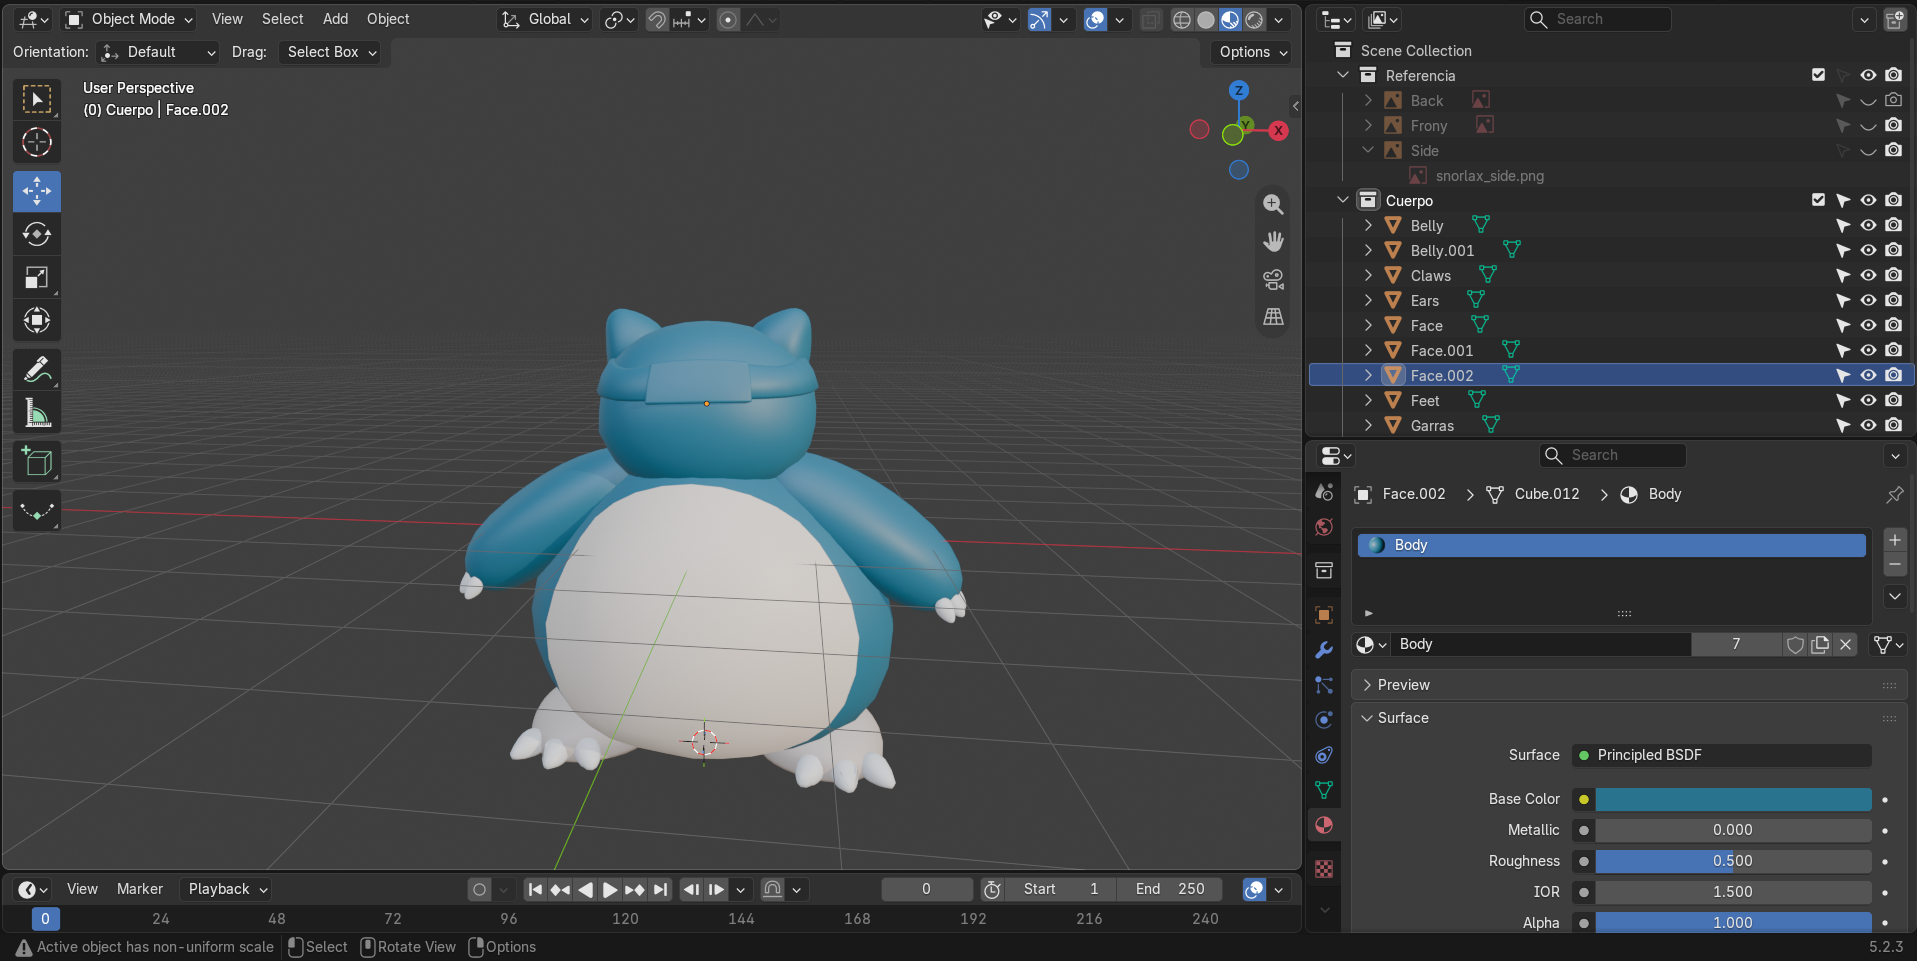
\includegraphics[width=\linewidth]{46_material_body_blue.png}
    \caption{Blue material.}
  \end{subfigure}\hfill
  \begin{subfigure}{0.32\linewidth}
    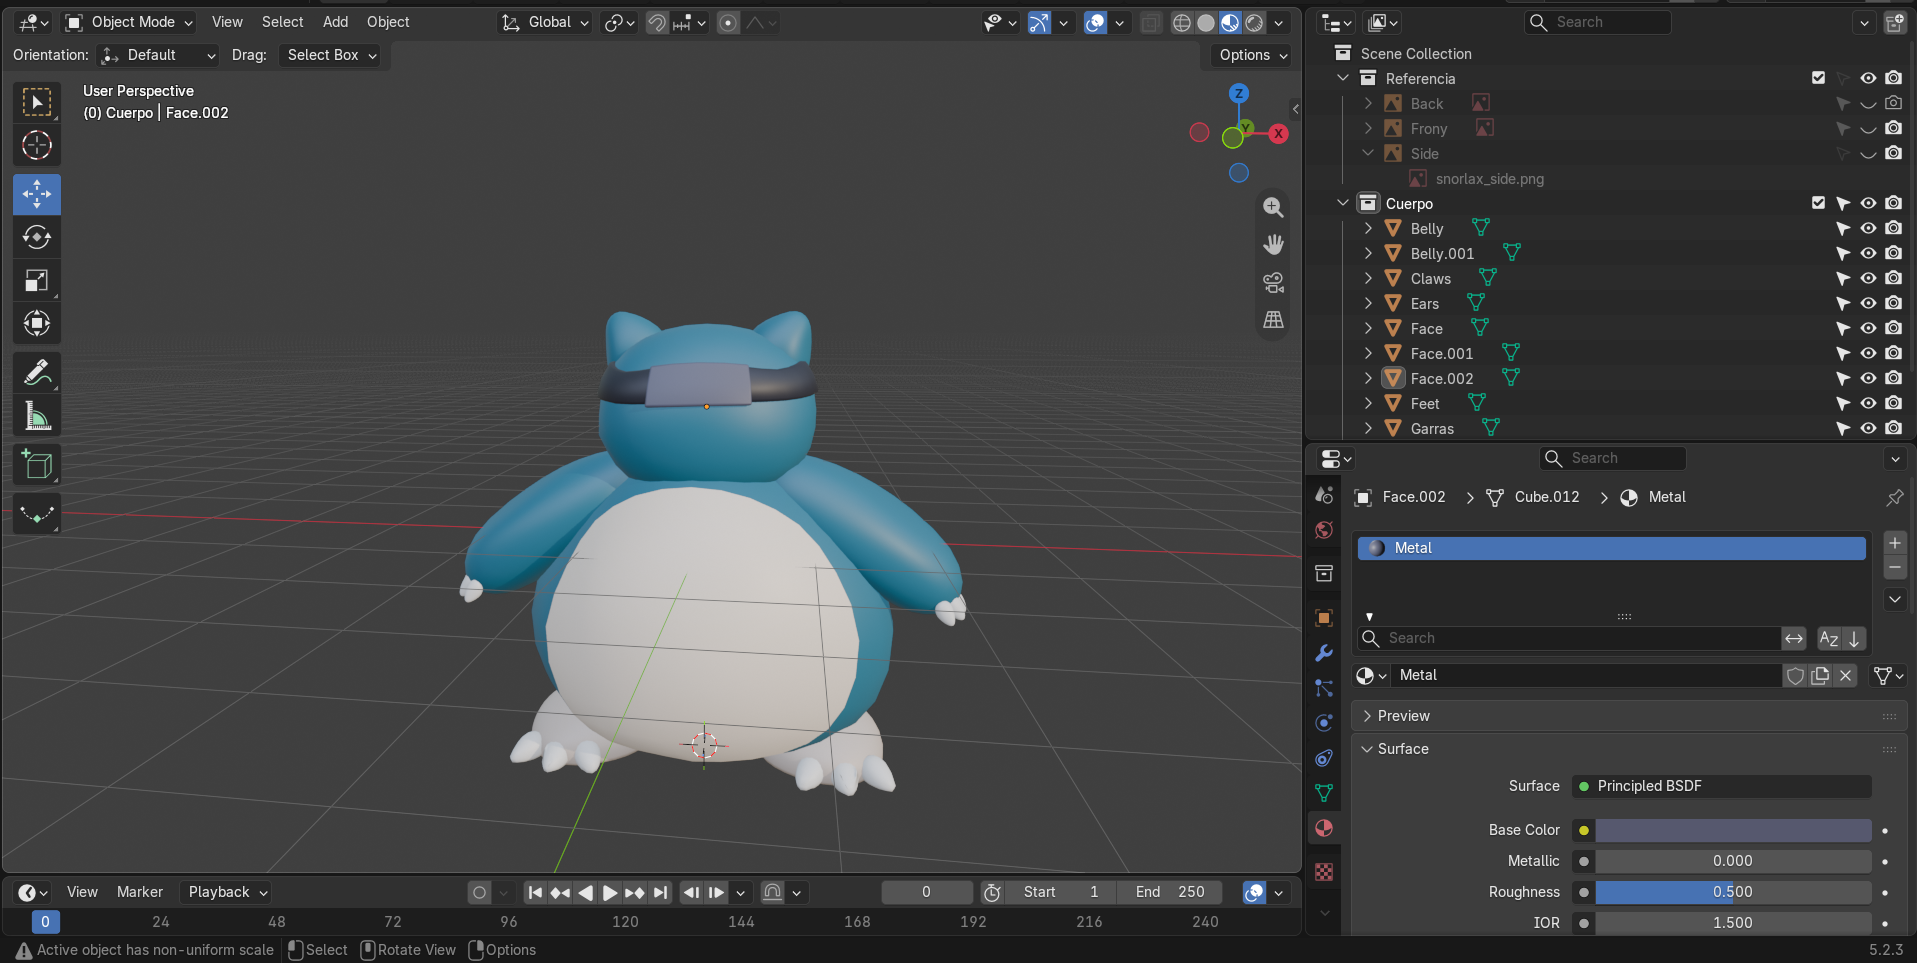
\includegraphics[width=\linewidth]{47_material_metal.png}
    \caption{Metal material.}
  \end{subfigure}
  \caption{Materials applied to the model.}
\end{figure}

%=====================================================================
\section{Headband}
%=====================================================================
\begin{enumerate}
  \item In Edit Mode, a horizontal ring of faces around the forehead of the
        head mesh was selected.
  \item These faces were duplicated and separated into a new object
        (\key{Shift+D}, \key{P} $\rightarrow$ \menu{Selection}). Because the
        band was created from the head itself, it follows the curvature of
        the head perfectly.
  \item A \textbf{Solidify} modifier gave the band thickness, and a
        \textbf{Bevel} modifier rounded its edges.
  \item A separate block was modeled in front for the metal plate and given
        the \emph{Metal} material.
\end{enumerate}

\fig{48_headband_faces_selected.png}{0.75}{Faces of the head selected to create the headband.}

\begin{figure}[H]
  \centering
  \begin{subfigure}{0.48\linewidth}
    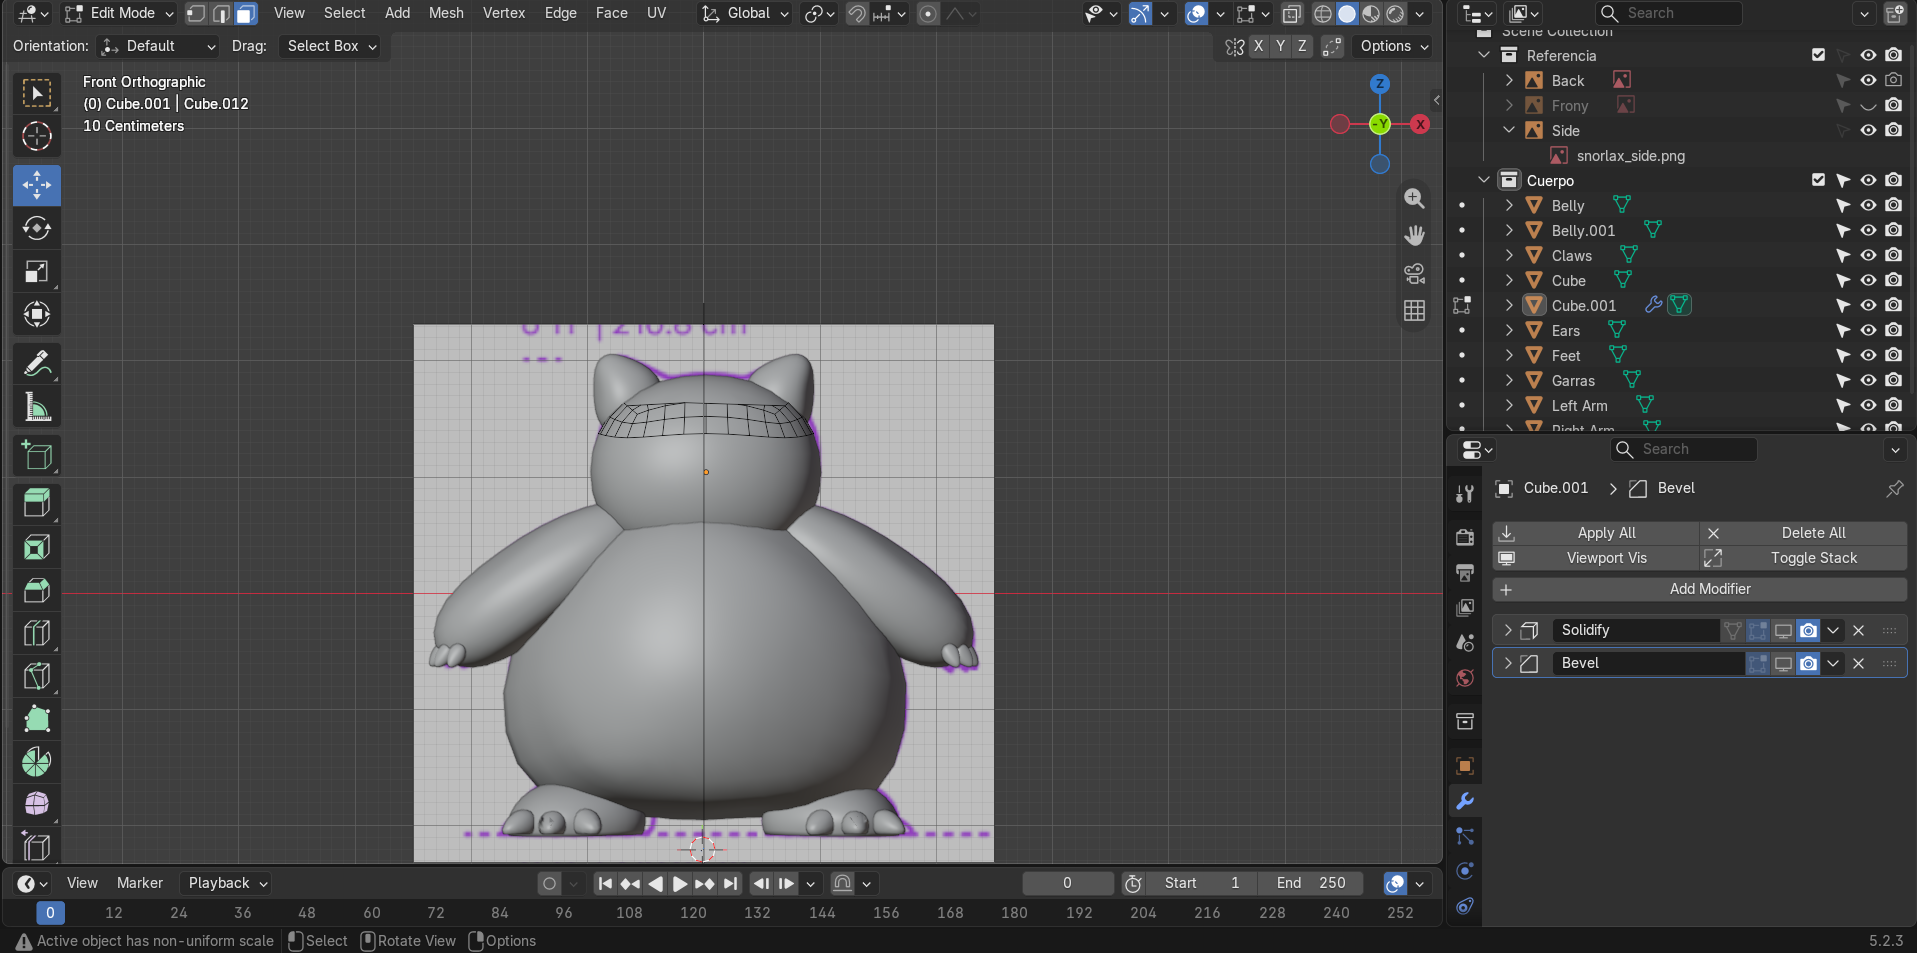
\includegraphics[width=\linewidth]{49_headband_solidify_bevel.png}
    \caption{Solidify and Bevel modifiers.}
  \end{subfigure}\hfill
  \begin{subfigure}{0.48\linewidth}
    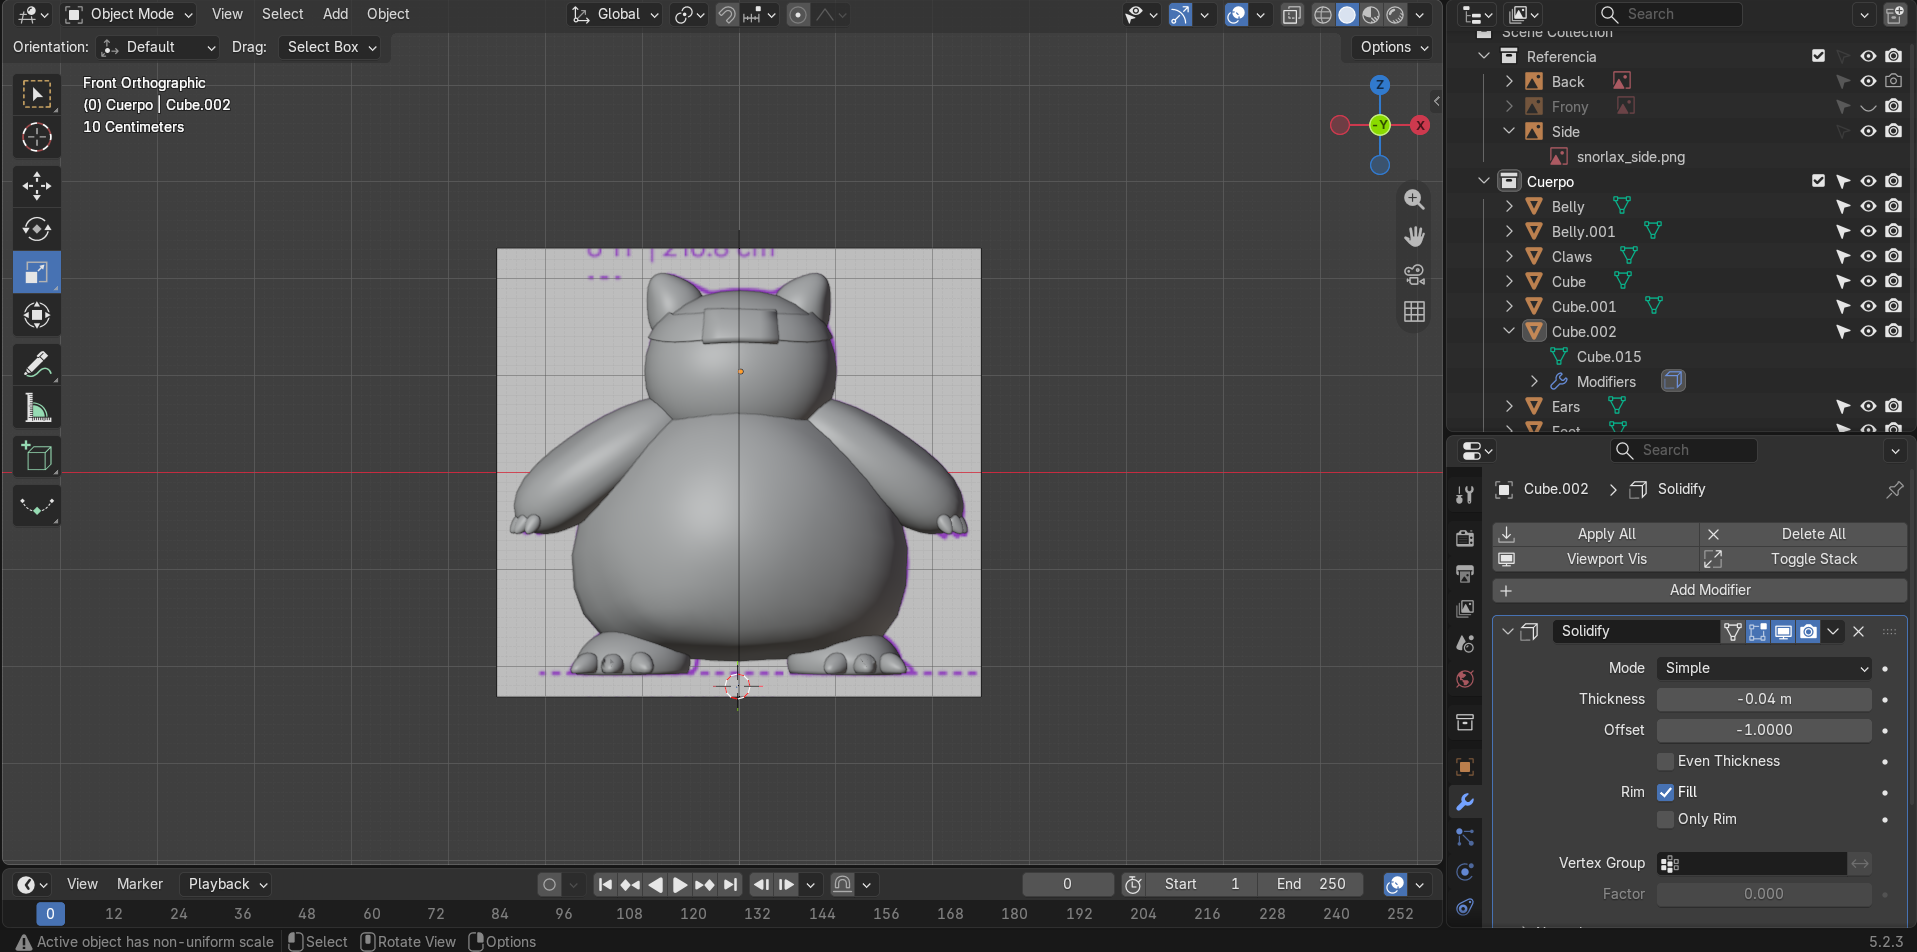
\includegraphics[width=\linewidth]{51_headband_solidify_settings.png}
    \caption{Solidify settings.}
  \end{subfigure}
  \caption{Headband.}
\end{figure}

%=====================================================================
\section{Eyes}
%=====================================================================
The eyes are thin curved strips that must sit exactly on the curved surface
of the face.

\begin{enumerate}
  \item A plane was added, rotated to face the front and shaped in Edit
        Mode into a thin strip following the eye line of the reference.
  \item The plane was subdivided (\menu{right click $\rightarrow$
        Subdivide}) so it has enough vertices to bend. A plane with only
        four vertices cannot follow a curved surface.
  \item Scale and rotation were applied (\key{Ctrl+A} $\rightarrow$
        \menu{All Transforms}) so the modifiers calculate thickness and
        direction correctly.
  \item A \textbf{Shrinkwrap} modifier was added with the head as
        \emph{Target}, \emph{Wrap Method: Project} along the Y axis
        (positive and negative) and an \emph{Offset} of 0.004\,m so the strip rests on the skin
        without sinking in.
  \item A \textbf{Solidify} modifier (thickness 0.03\,m, offset $+1$) gave
        it volume towards the outside of the face.
  \item The modifier order was set to
        \emph{Subdivision $\rightarrow$ Shrinkwrap $\rightarrow$ Solidify}:
        the strip is first smoothed, then wrapped onto the face, and only
        then thickened.
\end{enumerate}

\begin{figure}[H]
  \centering
  \begin{subfigure}{0.48\linewidth}
    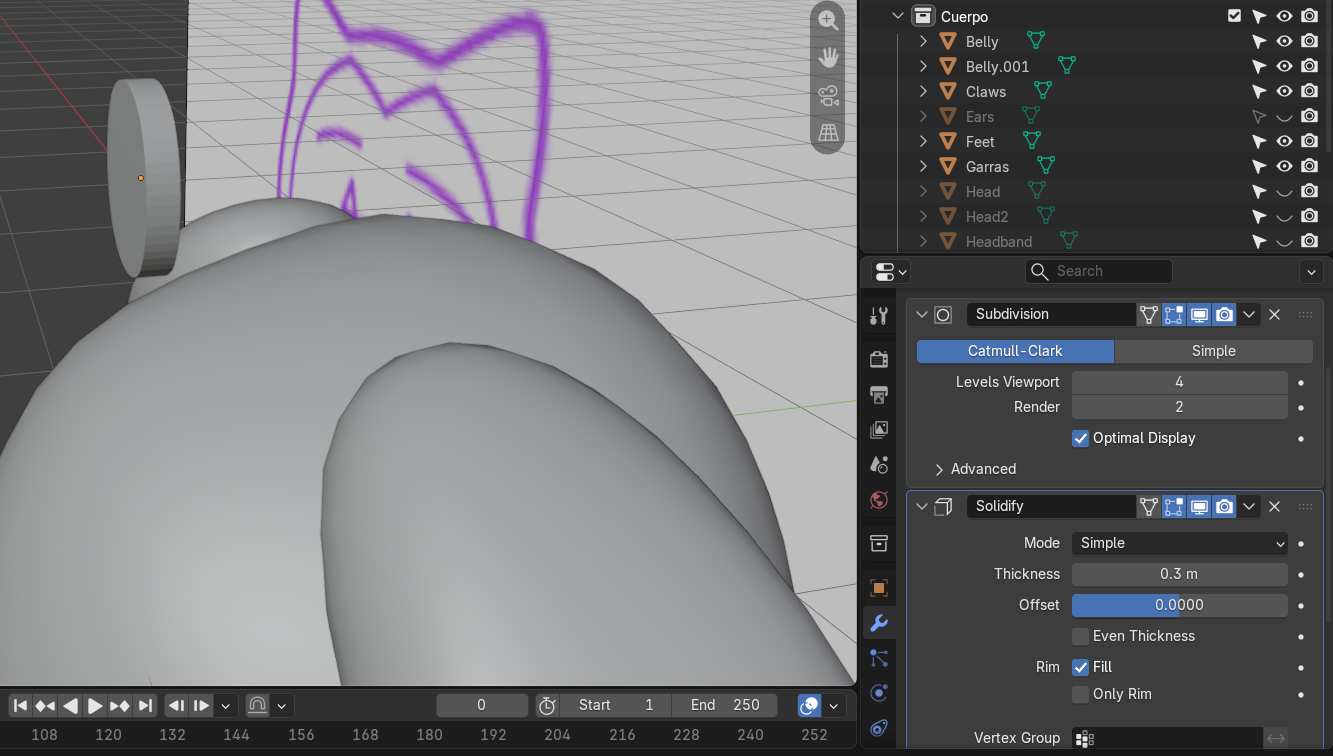
\includegraphics[width=\linewidth]{53_eye_plane_modifiers.png}
    \caption{Eye plane with Subdivision and Solidify.}
  \end{subfigure}\hfill
  \begin{subfigure}{0.48\linewidth}
    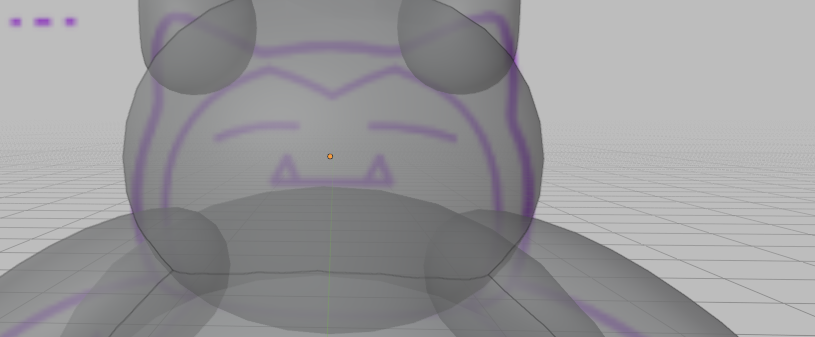
\includegraphics[width=\linewidth]{56_eye_pieces_xray.png}
    \caption{X-Ray view to align with the reference.}
  \end{subfigure}
  \caption{Preparing the eyes.}
\end{figure}

\begin{figure}[H]
  \centering
  \begin{subfigure}{0.48\linewidth}
    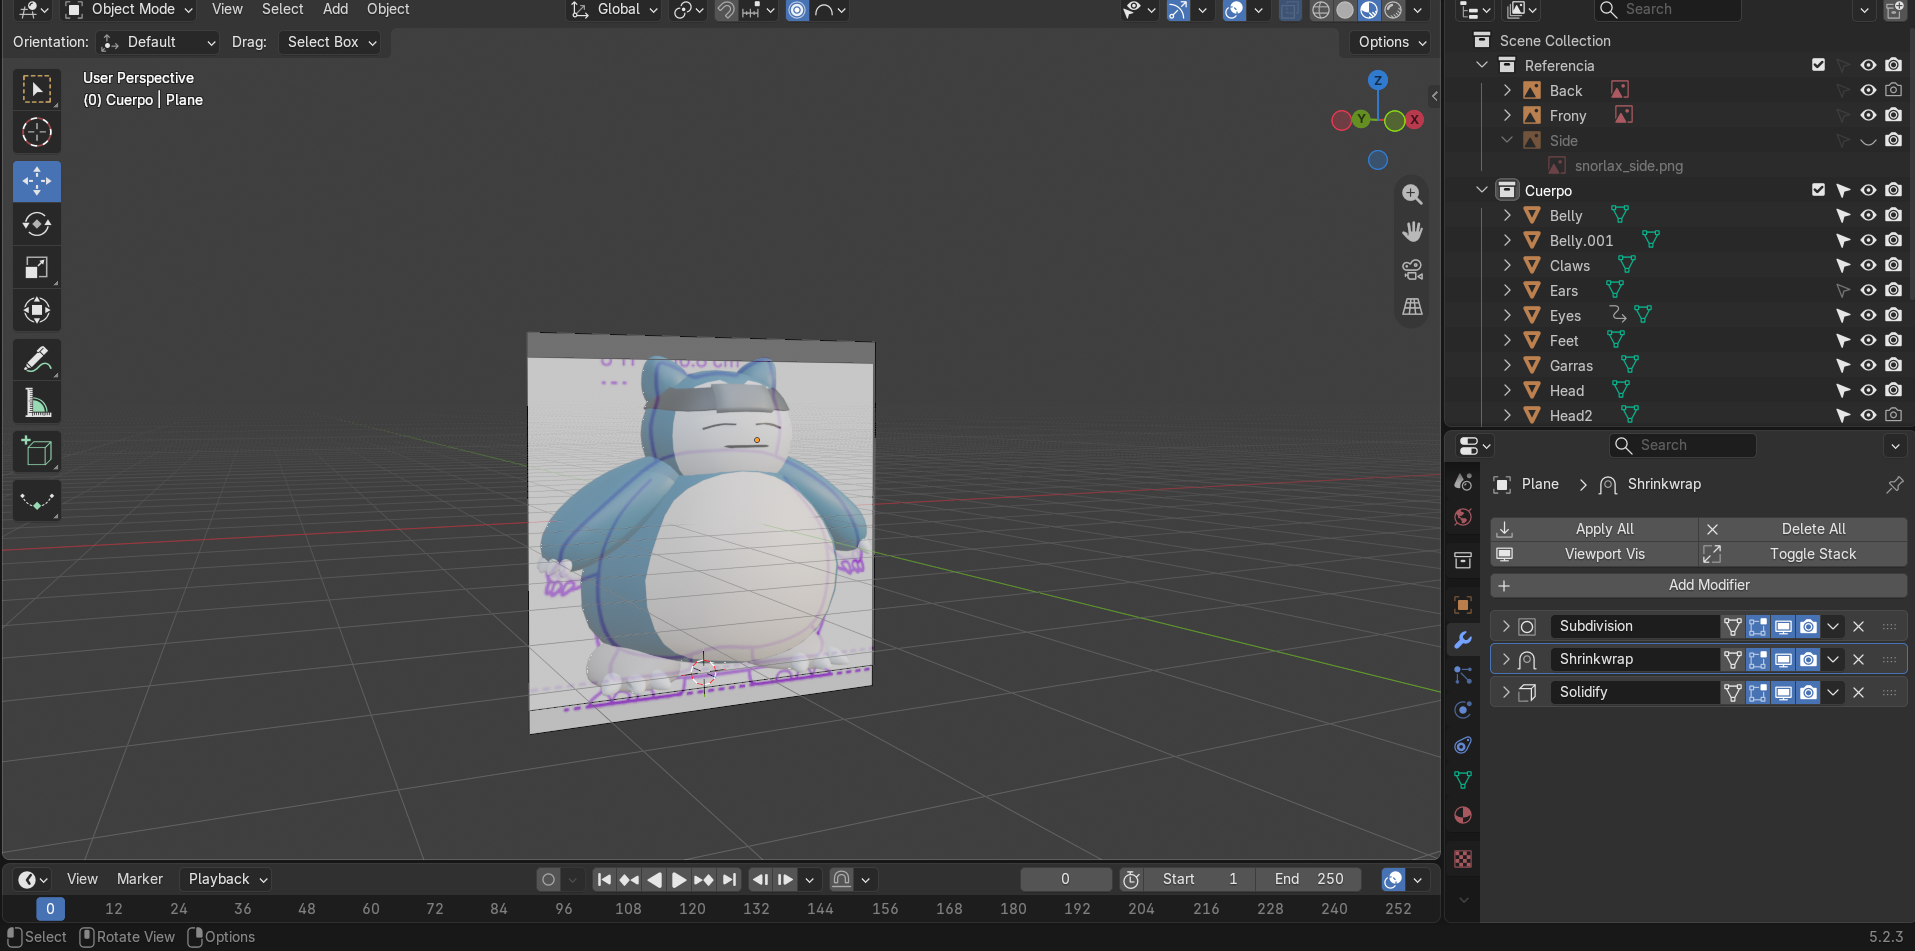
\includegraphics[width=\linewidth]{58_eyes_shrinkwrap.png}
    \caption{Shrinkwrap modifier added.}
  \end{subfigure}\hfill
  \begin{subfigure}{0.48\linewidth}
    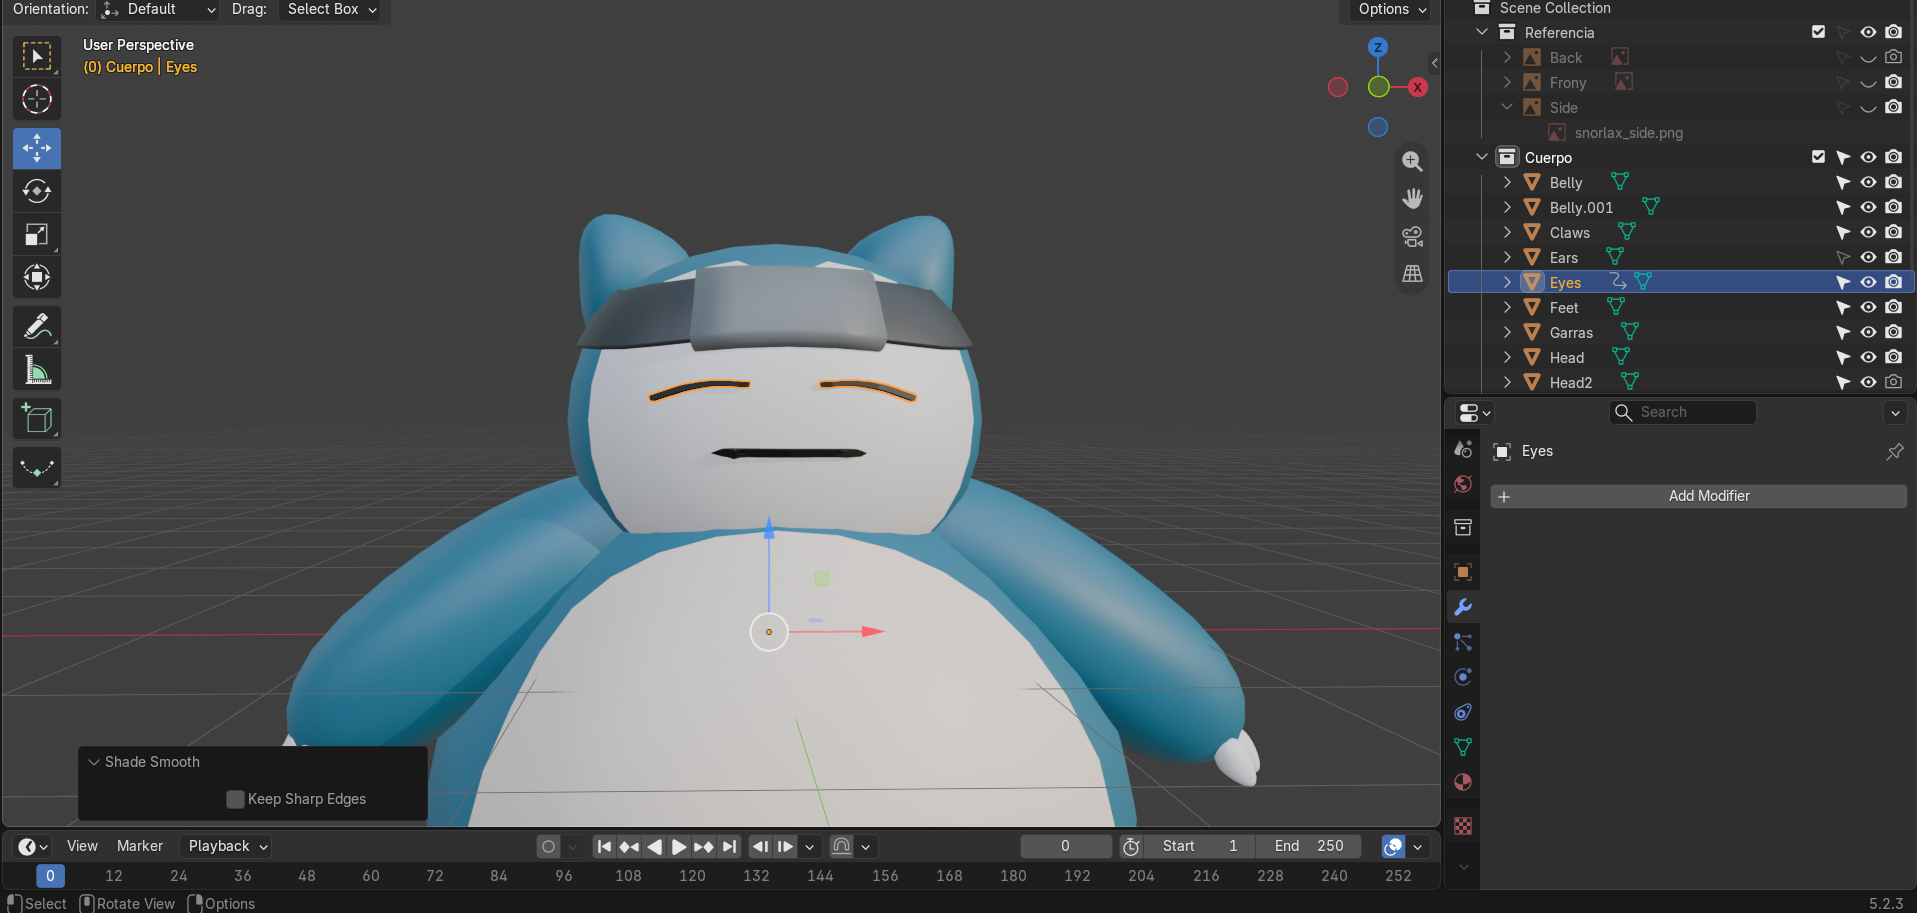
\includegraphics[width=\linewidth]{59_eyes_result.png}
    \caption{Eyes resting on the face.}
  \end{subfigure}
  \caption{Eyes.}
\end{figure}

%=====================================================================
\section{Mouth and fangs}
%=====================================================================
\begin{enumerate}
  \item The mouth was made the same way as the eyes: a thin subdivided
        strip with Subdivision, Shrinkwrap (target: head) and Solidify.
  \item The two fangs were made from cones with \emph{Radius 2} set to 0 so
        they end in a point. They were scaled, placed at the edge of the
        mouth and rotated so they point outward, following the angle of the
        face.
  \item \menu{Shade Auto Smooth} was applied to all the face pieces.
\end{enumerate}

\begin{figure}[H]
  \centering
  \begin{subfigure}{0.48\linewidth}
    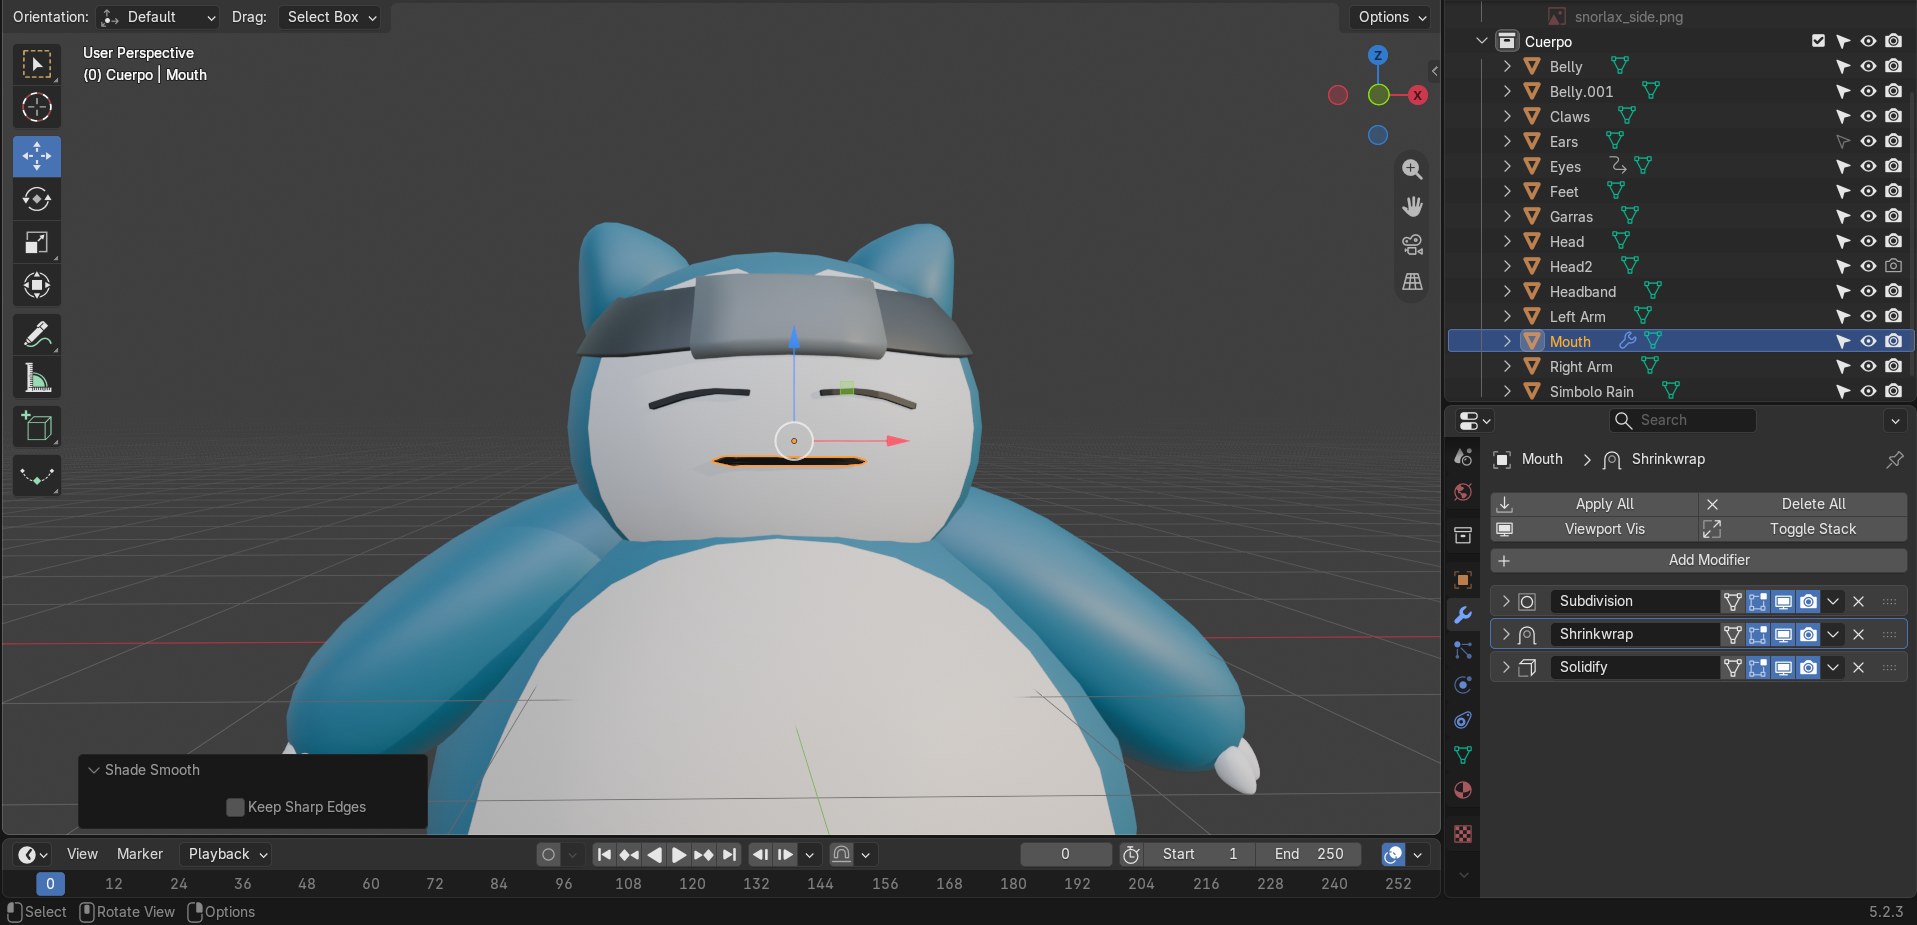
\includegraphics[width=\linewidth]{60_mouth_shrinkwrap.png}
    \caption{Mouth with Shrinkwrap.}
  \end{subfigure}\hfill
  \begin{subfigure}{0.48\linewidth}
    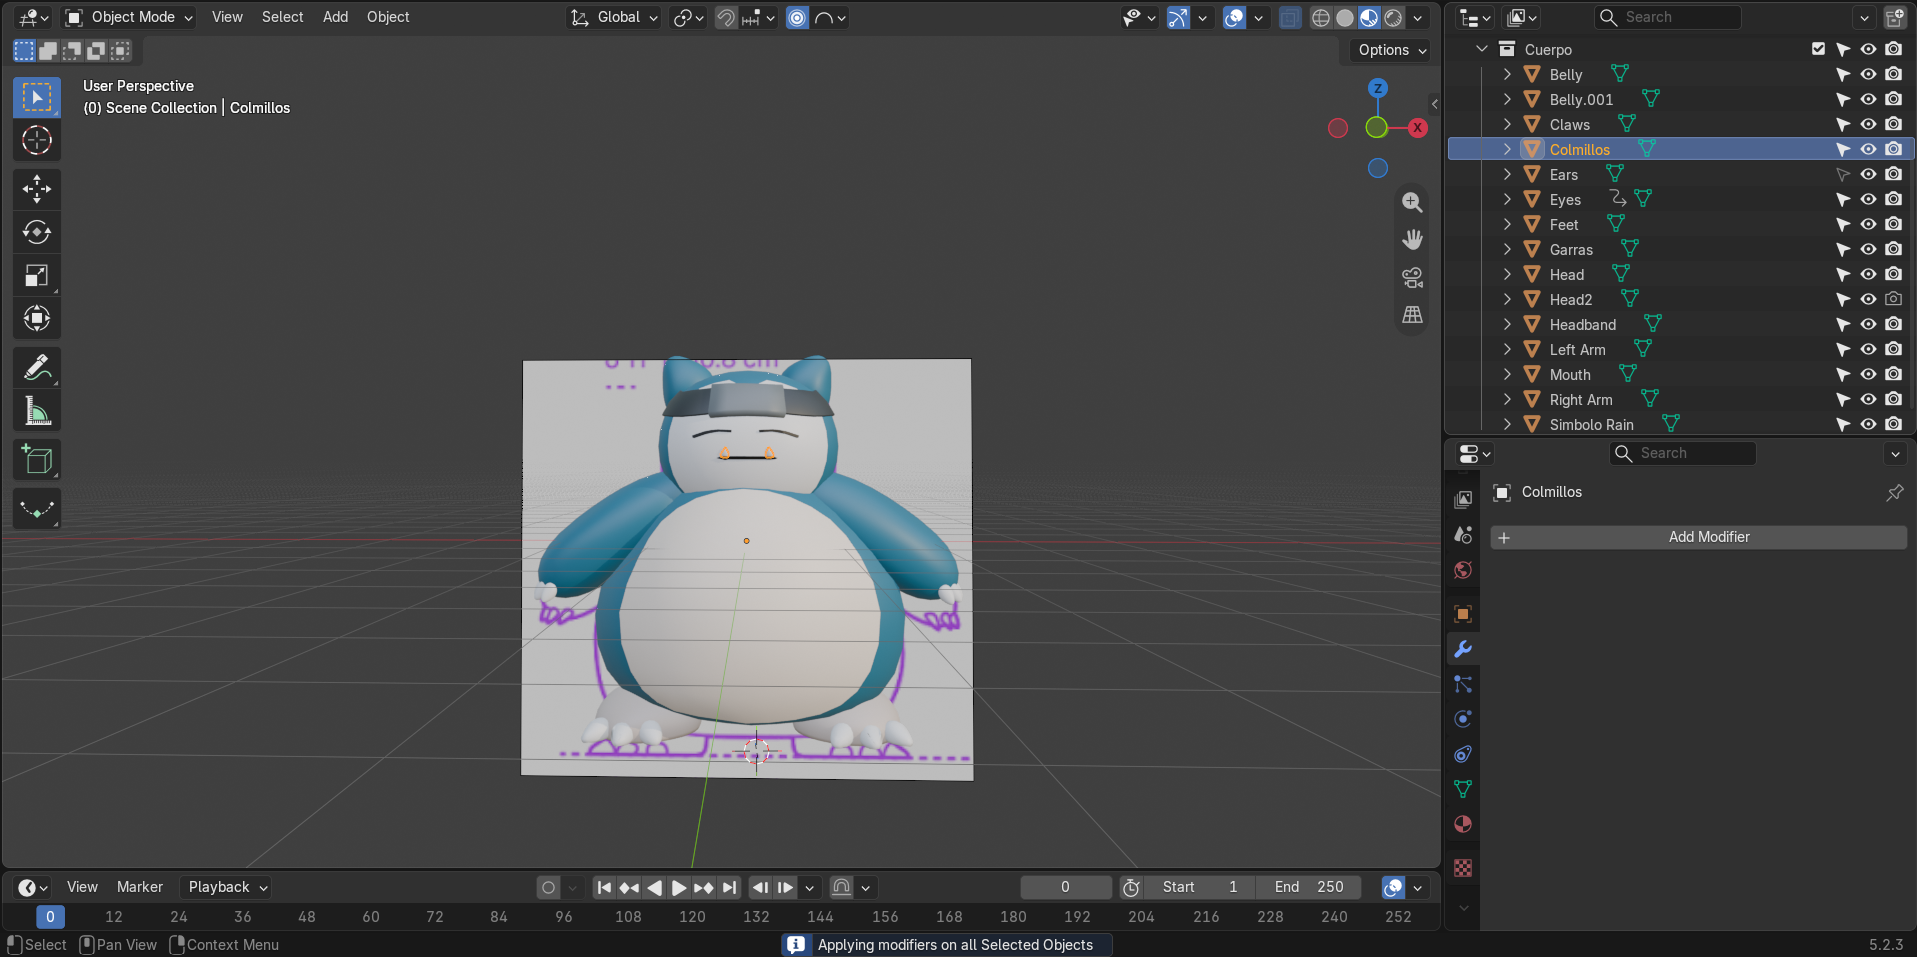
\includegraphics[width=\linewidth]{62_fangs_added.png}
    \caption{Fangs added.}
  \end{subfigure}
  \caption{Mouth and fangs.}
\end{figure}

\fig{63_face_result.png}{0.65}{Finished face: eyes, mouth and fangs.}

%=====================================================================
\section{Headband plate symbol}
%=====================================================================
The symbol on the plate was made with a ``pixel'' technique: a grid sheet
that is already wrapped onto the plate, from which the unneeded squares are
deleted.

\begin{enumerate}
  \item A grid plane (\emph{Lamina\_Dibujo}) of $42\times22$ squares was
        placed in front of the plate.
  \item It received a \textbf{Shrinkwrap} modifier with the plate as target
        (\emph{Nearest Surface Point}, \emph{Outside Surface}, offset
        0.003\,m) and a \textbf{Solidify} modifier (0.012\,m) so it follows
        the curvature of the plate and has relief.
  \item In Edit Mode, front view (\key{Numpad 1}) and face selection
        (\key{3}), the squares that form the symbol were selected: the
        circle-select tool (\key{C}) for free shapes and
        \key{Ctrl+click} (shortest path) for straight lines.
  \item The selection was inverted (\key{Ctrl+I}) and the remaining squares
        were deleted (\key{X} $\rightarrow$ \menu{Faces}). Only the symbol
        remains, already curved and with thickness.
\end{enumerate}

\begin{figure}[H]
  \centering
  \begin{subfigure}{0.48\linewidth}
    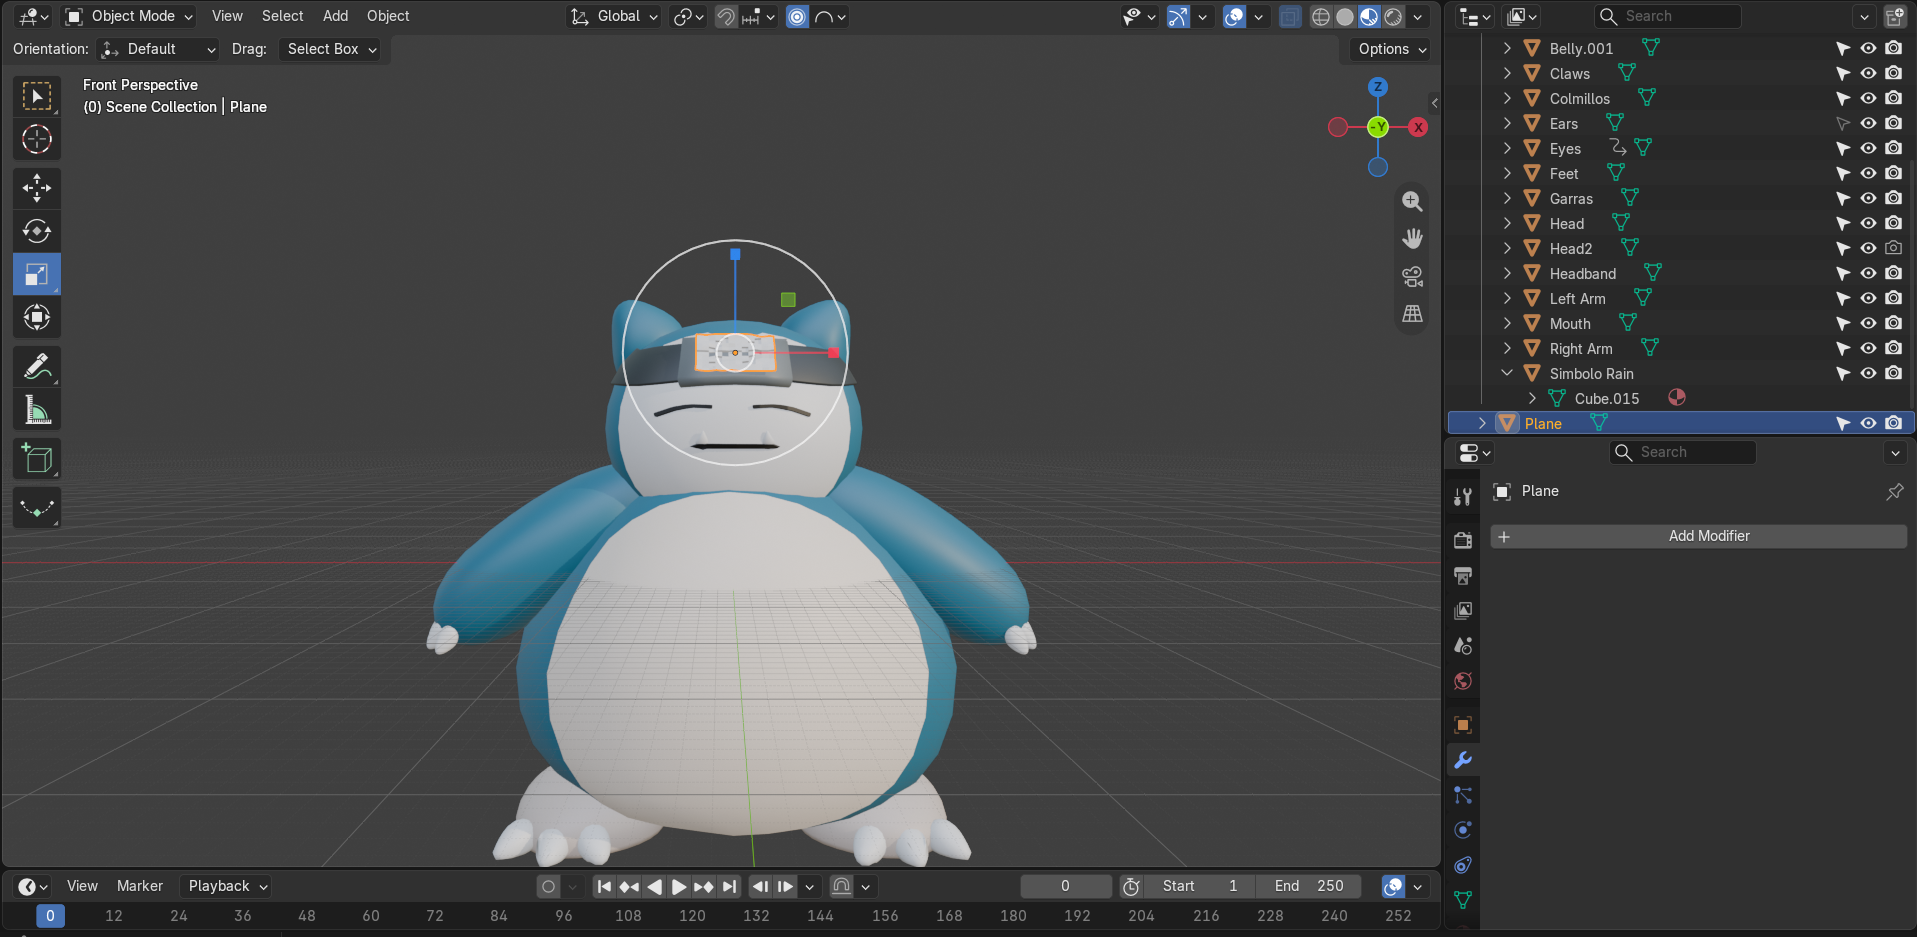
\includegraphics[width=\linewidth]{64_plate_sheet_added.png}
    \caption{Grid sheet on the plate.}
  \end{subfigure}\hfill
  \begin{subfigure}{0.48\linewidth}
    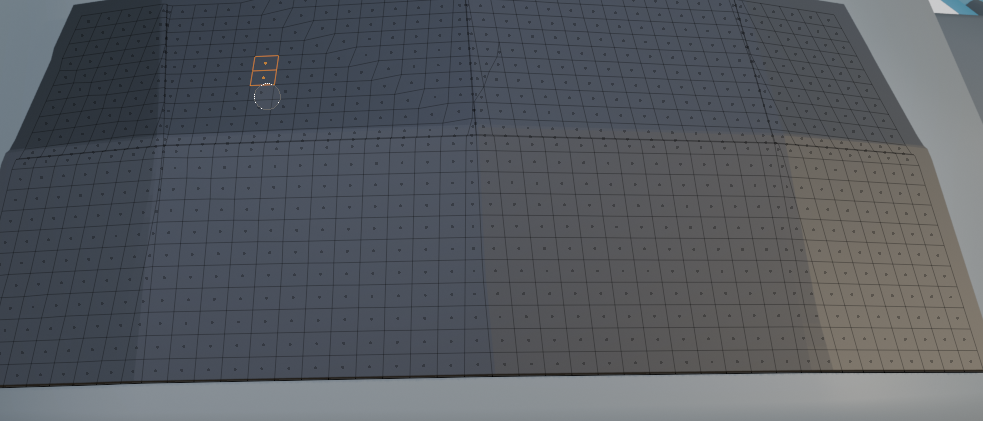
\includegraphics[width=\linewidth]{65_plate_grid.png}
    \caption{Close-up of the grid.}
  \end{subfigure}
  \caption{Preparing the symbol sheet.}
\end{figure}

\begin{figure}[H]
  \centering
  \begin{subfigure}{0.48\linewidth}
    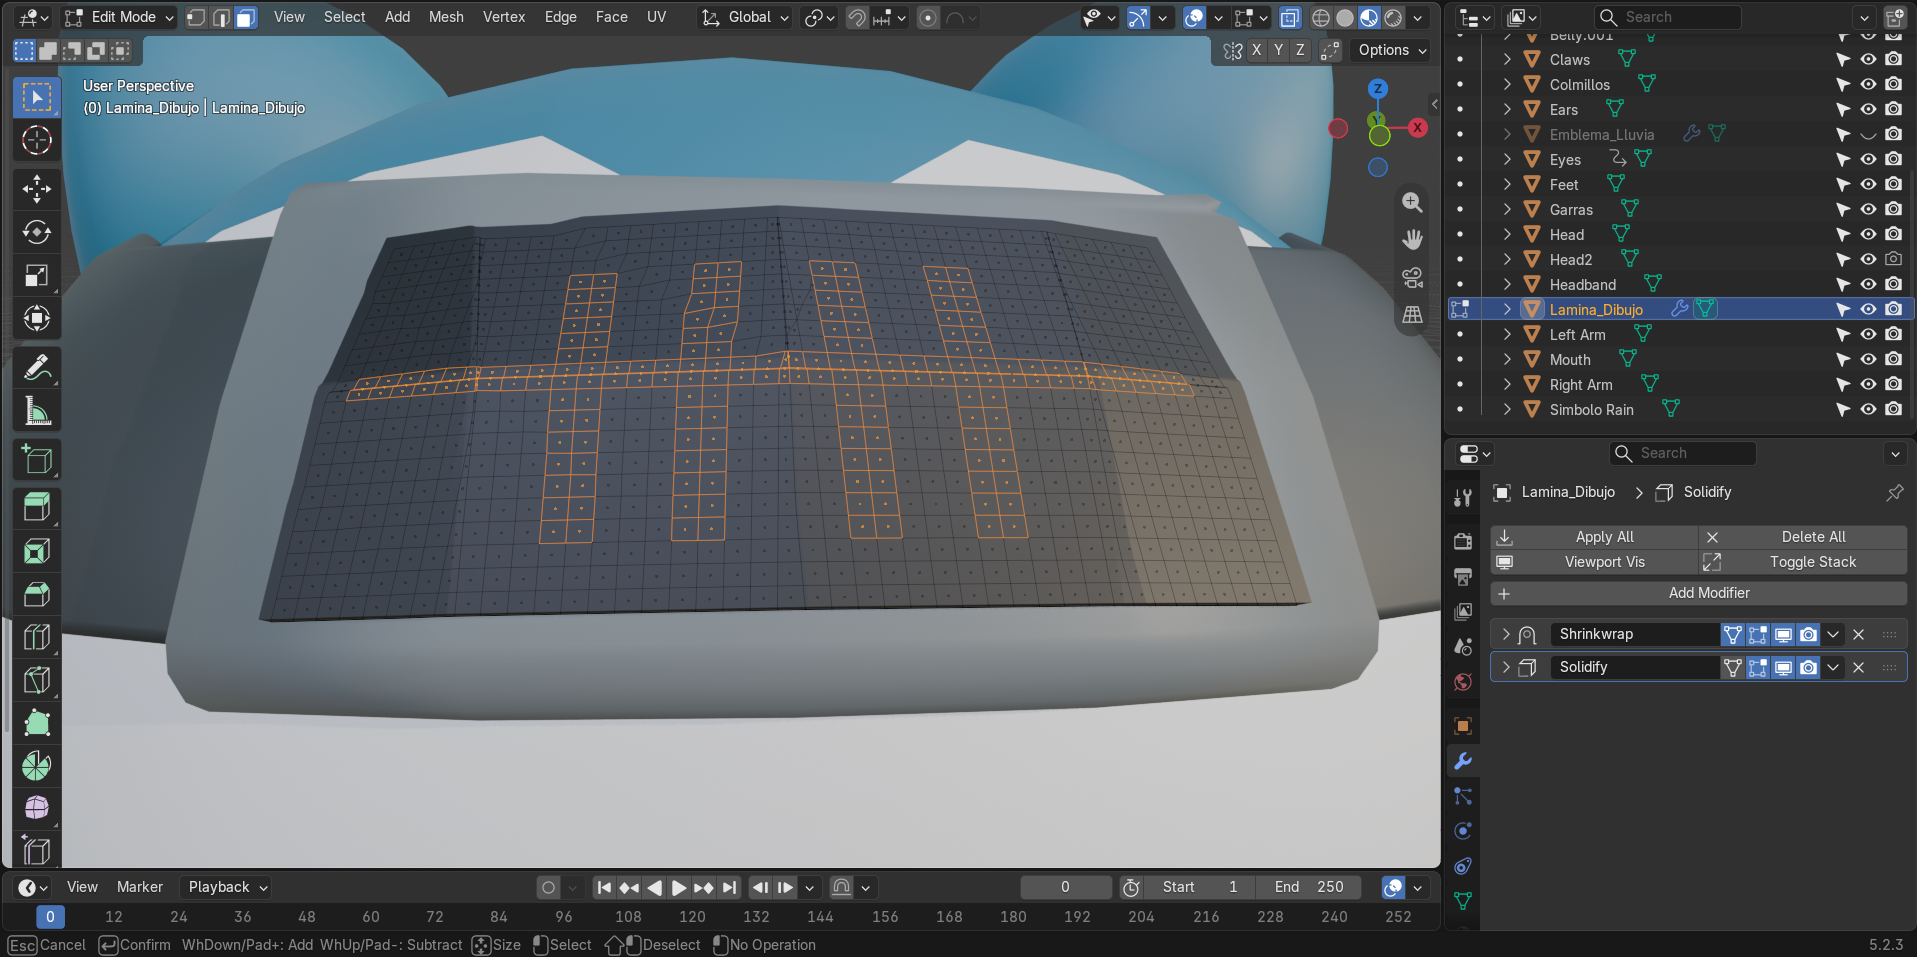
\includegraphics[width=\linewidth]{66_symbol_faces_selected.png}
    \caption{Symbol squares selected.}
  \end{subfigure}\hfill
  \begin{subfigure}{0.48\linewidth}
    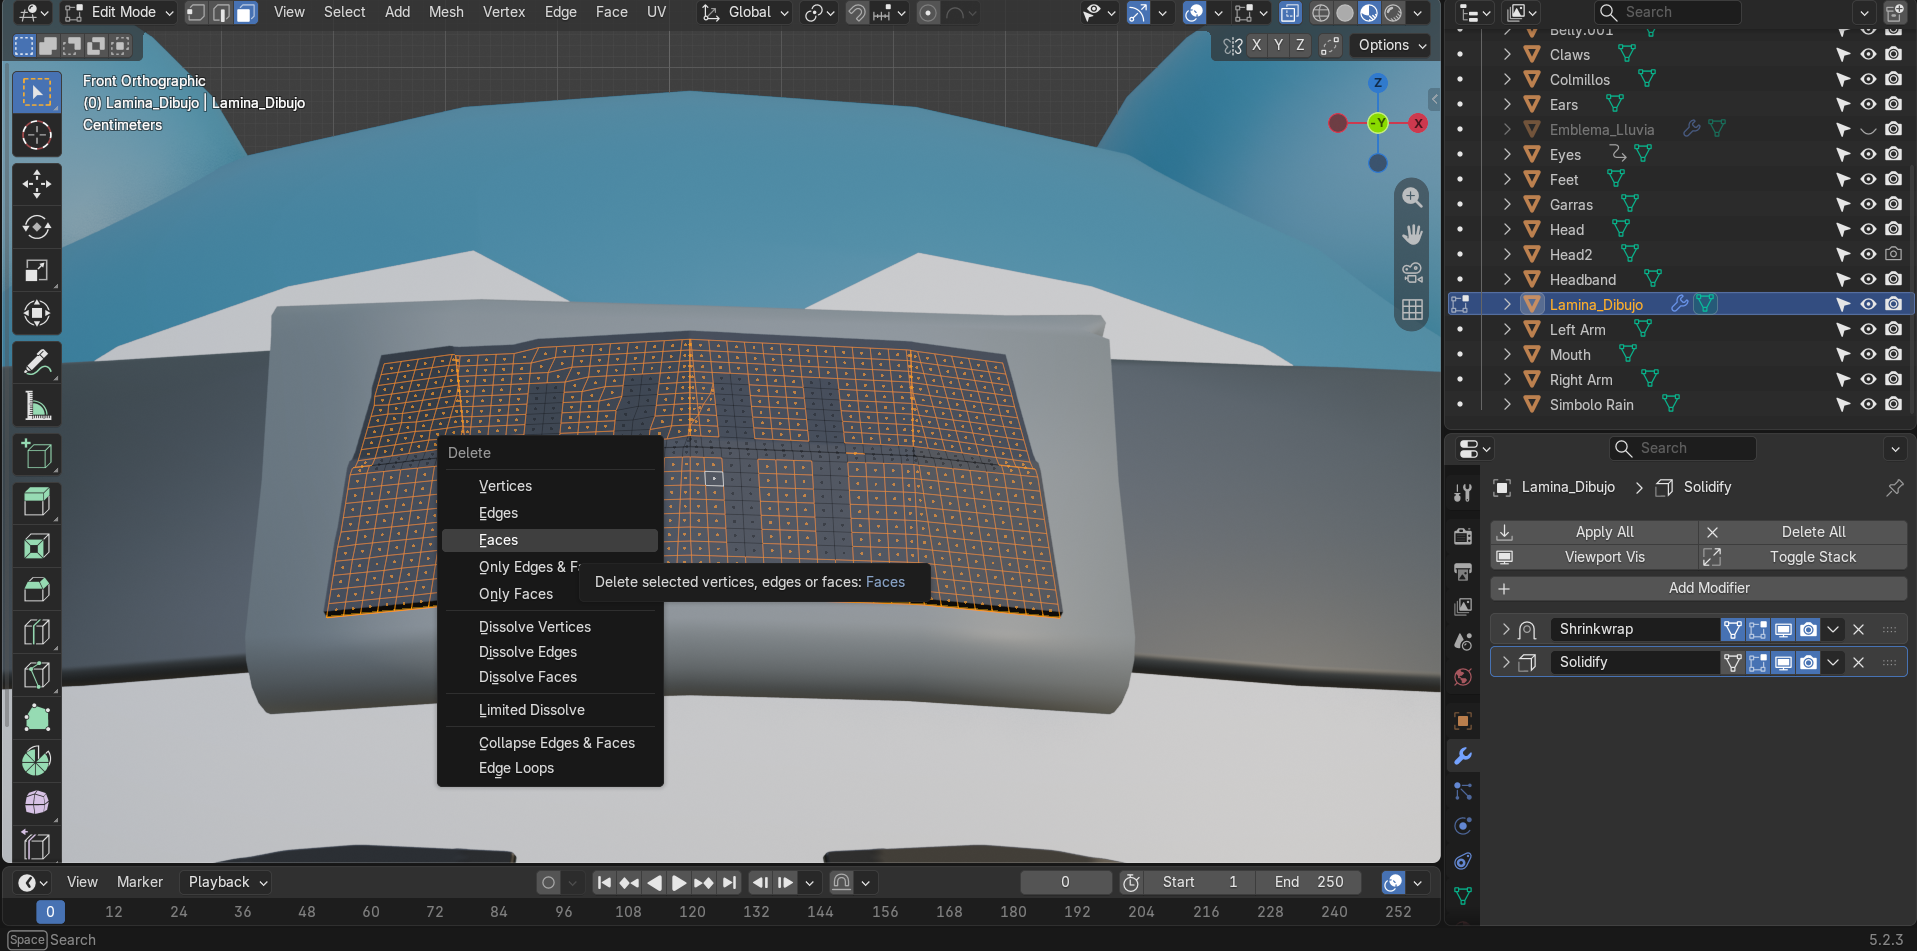
\includegraphics[width=\linewidth]{68_symbol_delete_faces.png}
    \caption{Deleting the inverted selection.}
  \end{subfigure}
  \caption{Drawing the symbol.}
\end{figure}

\fig{70_symbol_result_edit_mode.png}{0.85}{Finished symbol on the plate (Edit Mode, front view).}

%=====================================================================
\section{Rivets}
%=====================================================================
Rivets were added at both ends of the plate as separate objects, so the plate
mesh did not need to be modified.

\begin{enumerate}
  \item A UV sphere (16 segments, 8 rings, small radius) was added and
        flattened along its depth axis so it looks like a rivet head.
  \item \menu{Shade Auto Smooth} and the \emph{Metal} material were applied,
        and the transforms were applied (\key{Ctrl+A}).
  \item Snapping was enabled (\key{Shift+Tab}) with \emph{Snap To: Face
        Project} and \emph{Align Rotation to Target}, so that moving the
        rivet with \key{G} makes it stick to the plate and orient itself to
        the surface.
  \item The rivet was duplicated (\key{Shift+D}) to form a vertical column
        of three, and the copies were joined into one object (\key{Ctrl+J}).
  \item A \textbf{Mirror} modifier with the plate as \emph{Mirror Object}
        created the column on the opposite end symmetrically.
\end{enumerate}

\begin{figure}[H]
  \centering
  \begin{subfigure}{0.48\linewidth}
    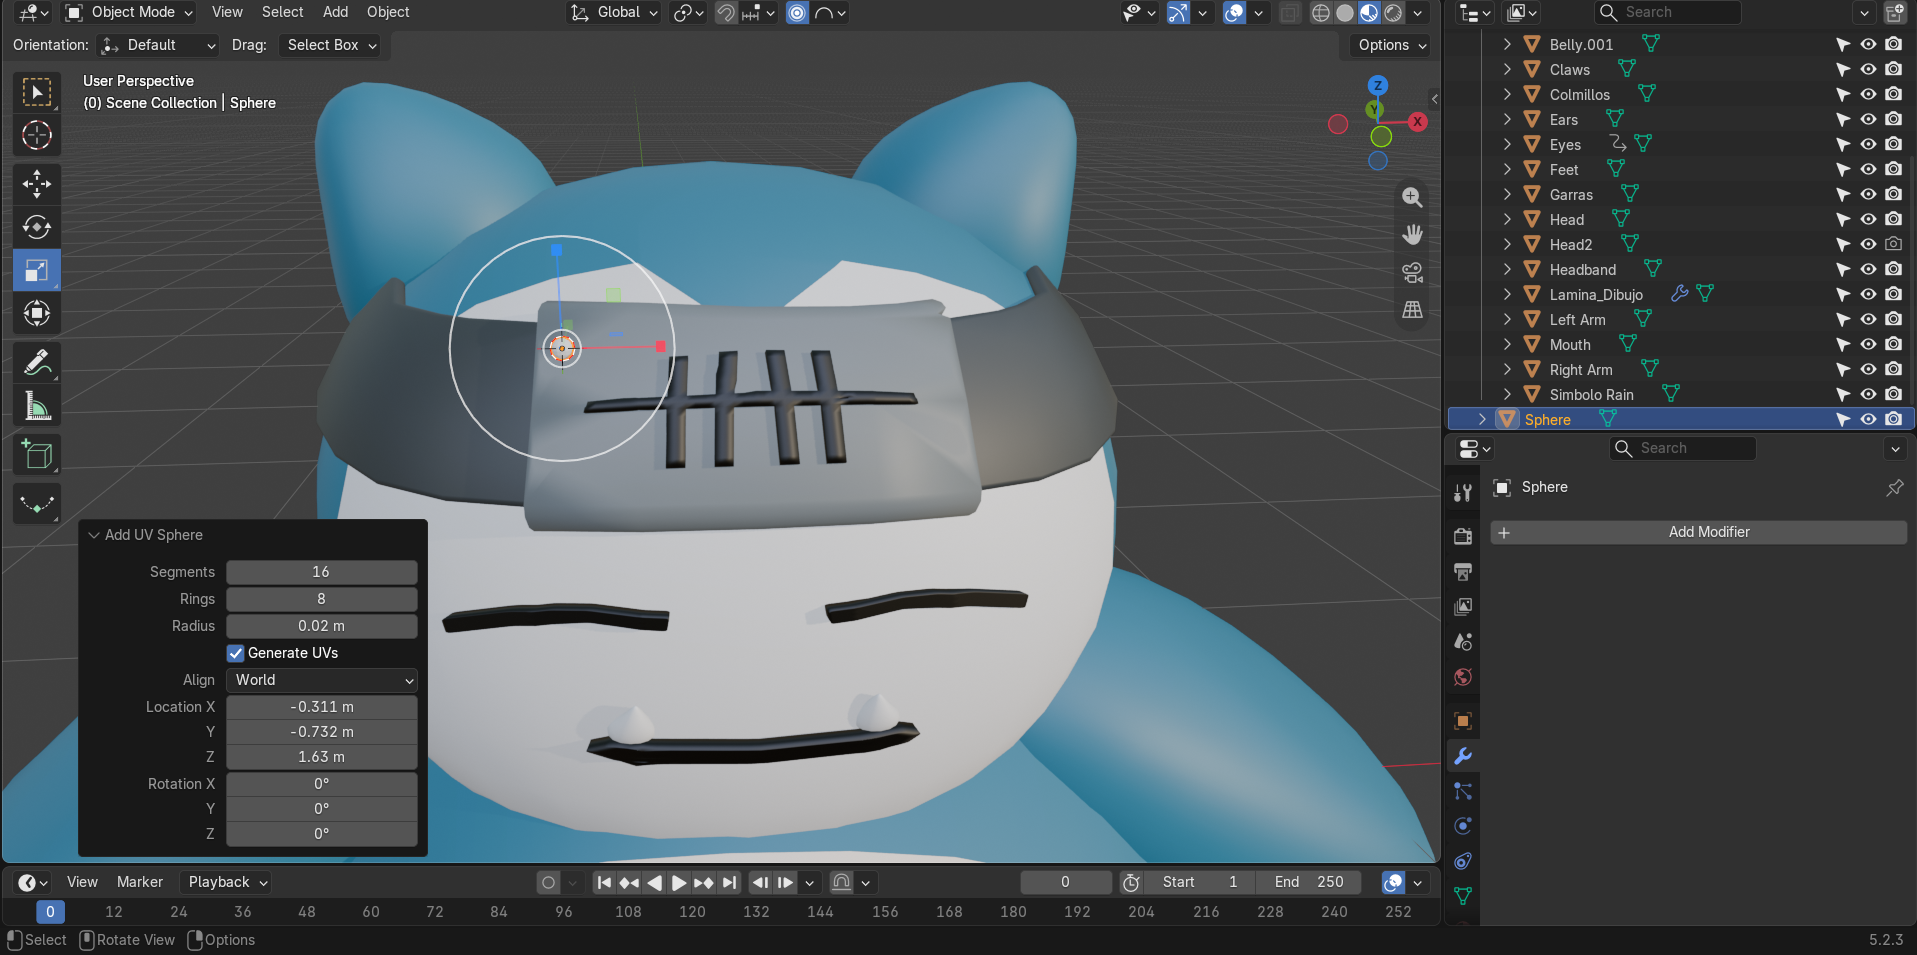
\includegraphics[width=\linewidth]{73_rivet_uv_sphere.png}
    \caption{UV sphere for the rivet.}
  \end{subfigure}\hfill
  \begin{subfigure}{0.48\linewidth}
    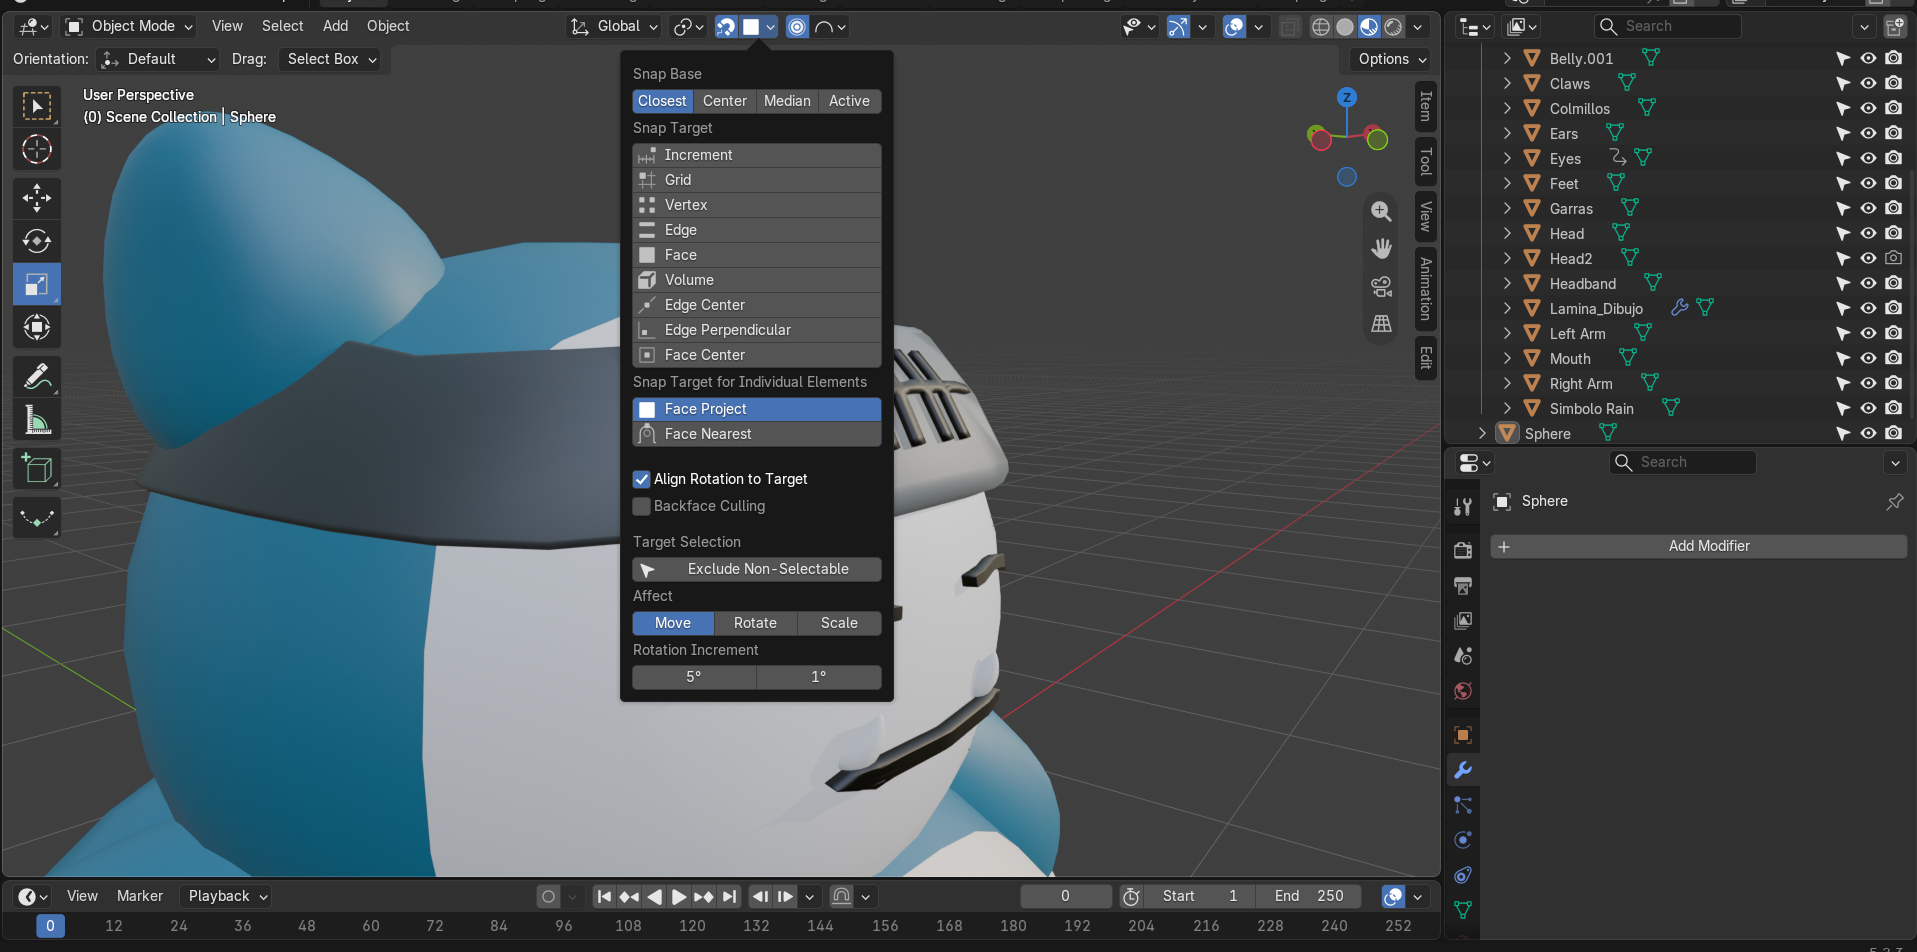
\includegraphics[width=\linewidth]{74_rivet_snapping.png}
    \caption{Snapping settings.}
  \end{subfigure}
  \caption{Creating and placing a rivet.}
\end{figure}

\begin{figure}[H]
  \centering
  \begin{subfigure}{0.48\linewidth}
    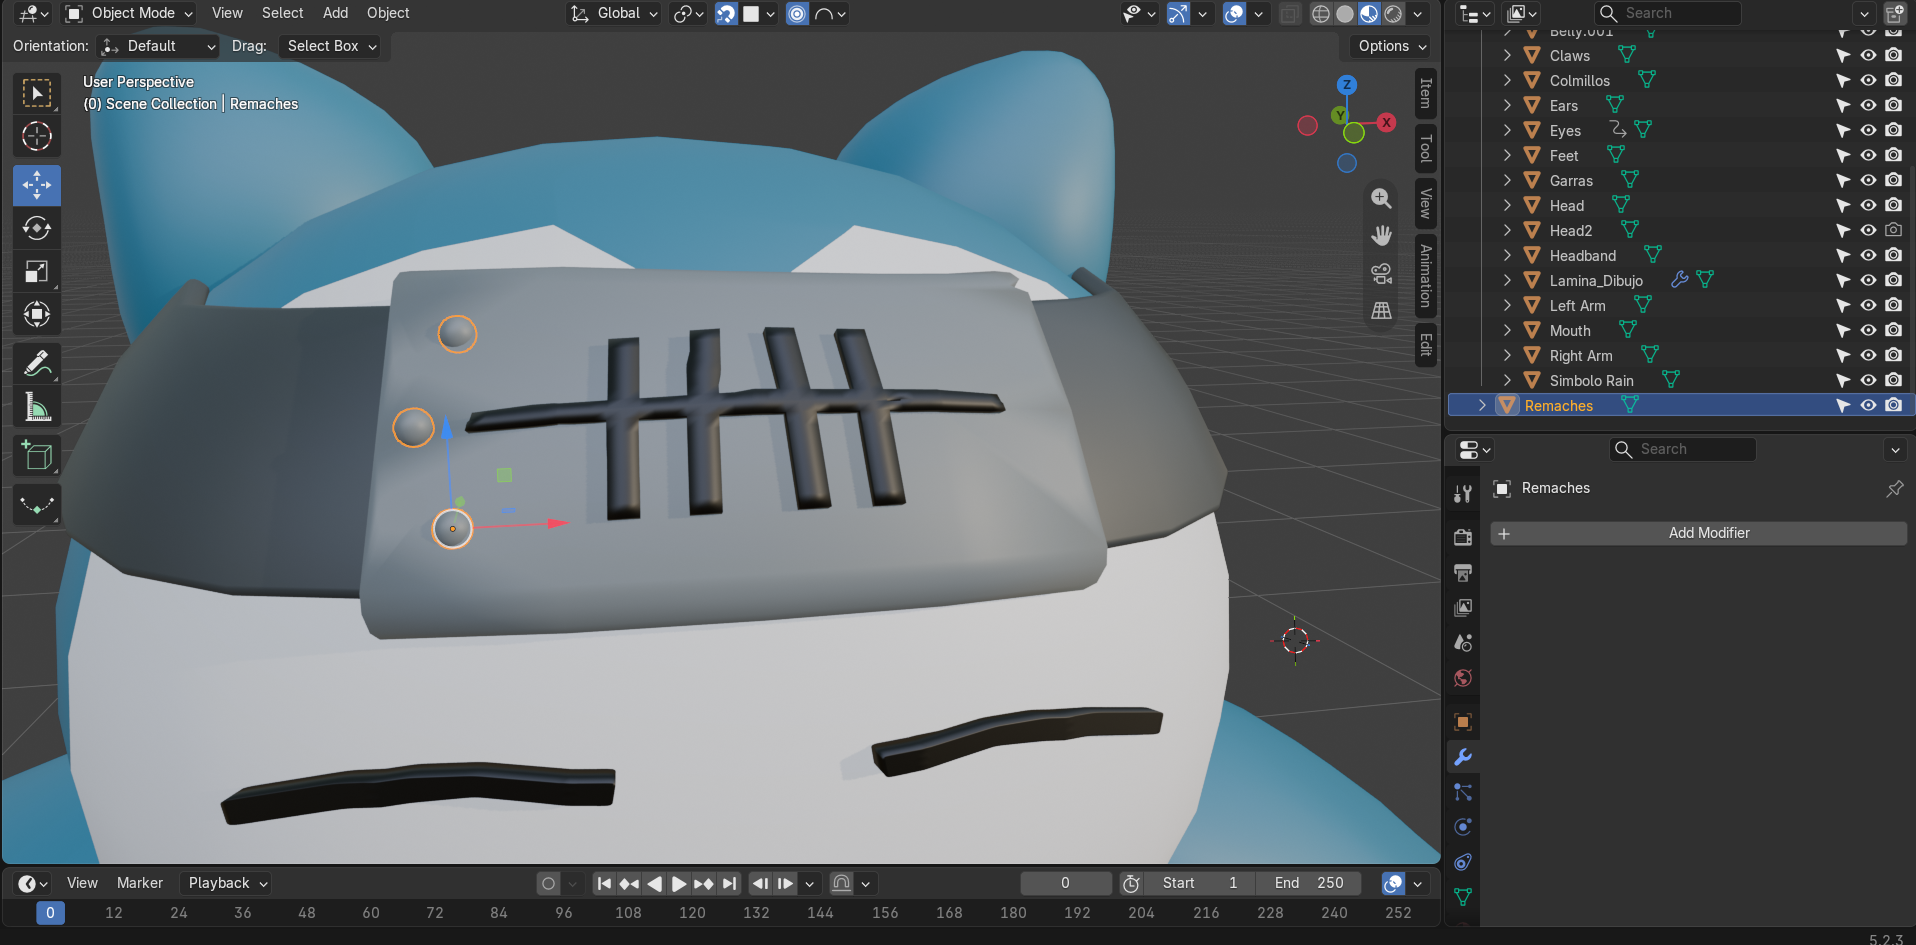
\includegraphics[width=\linewidth]{76_rivets_placed.png}
    \caption{Column of rivets.}
  \end{subfigure}\hfill
  \begin{subfigure}{0.48\linewidth}
    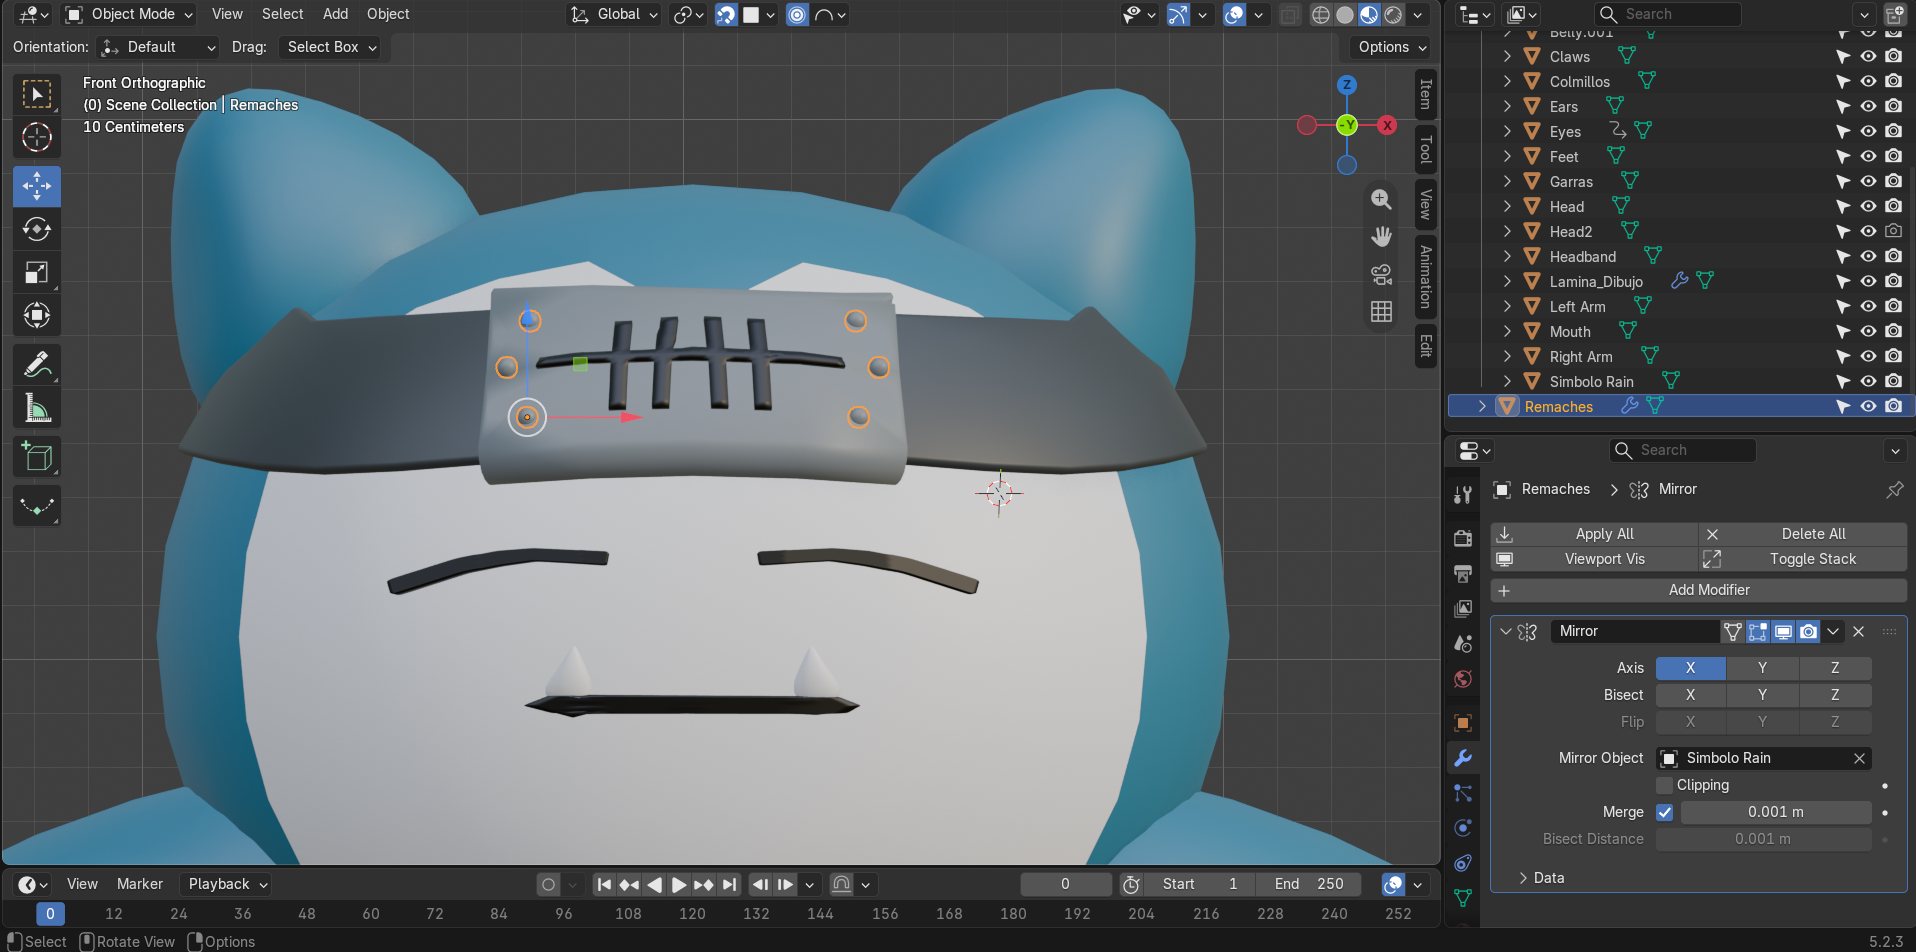
\includegraphics[width=\linewidth]{77_rivets_mirror_final.png}
    \caption{Mirror modifier: final result.}
  \end{subfigure}
  \caption{Rivets.}
\end{figure}

%=====================================================================
\section{Summary of tools and modifiers}
%=====================================================================
\begin{table}[H]
\centering
\begin{tabular}{@{}ll@{}}
\toprule
\textbf{Tool / modifier} & \textbf{Used for} \\
\midrule
Reference images        & Tracing proportions in front and side views \\
Sculpt Mode (Grab)      & Body, head and arm shapes \\
Extrude (\key{E})       & Claws on feet and hands \\
Separate (\key{P})      & Belly and headband from existing meshes \\
Mirror                  & Ears, feet, arms and rivets \\
Subdivision Surface     & Smooth, rounded surfaces \\
Solidify                & Thickness of headband, eyes, mouth and symbol \\
Bevel                   & Rounded edges of the headband \\
Shrinkwrap              & Eyes, mouth and symbol following curved surfaces \\
Snapping (Face Project) & Placing rivets on the plate \\
Shade Auto Smooth       & Smooth shading of the final pieces \\
\bottomrule
\end{tabular}
\caption{Main tools used in the project.}
\end{table}

\end{document}
